\begin{tikzpicture}[scale=.2, anchor=south west]
\node[draw=black, rectangle split, rectangle split parts=3] (sn0x8fd4380W-5) at (-5.5, -12) {
\begin{tikzpicture}[scale=.2]
\node[circle, scale=0.75, fill] (tid0) at (4.5,0){};
\node[circle, scale=0.75, fill] (tid1) at (2.25,1.5){};
\node[circle, scale=0.75, fill, red] (tid4) at (0.75,3){};
\node[circle, scale=0.75, fill, red] (tid5) at (2.25,3){};
\node[circle, scale=0.75, fill] (tid6) at (3.75,3){};
\draw[](tid1) -- (tid4);
\draw[](tid1) -- (tid5);
\draw[](tid1) -- (tid6);
\node[circle, scale=0.75, fill] (tid2) at (6,1.5){};
\node[circle, scale=0.75, fill] (tid7) at (5.25,3){};
\node[circle, scale=0.75, fill] (tid8) at (6.75,3){};
\draw[](tid2) -- (tid7);
\draw[](tid2) -- (tid8);
\node[circle, scale=0.75, fill] (tid3) at (8.25,1.5){};
\node[circle, scale=0.75, fill, red] (tid9) at (8.25,3){};
\draw[](tid3) -- (tid9);
\draw[](tid0) -- (tid1);
\draw[](tid0) -- (tid2);
\draw[](tid0) -- (tid3);

\end{tikzpicture}
\nodepart{two}
\footnotesize{5.20531}
\nodepart{three}
\footnotesize{$22\:44\:11\:22$}
};
\node[draw=black, rectangle split, rectangle split parts=3] (sn0x8fd3f88W-20) at (-20.5, -24) {
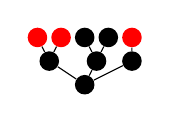
\begin{tikzpicture}[scale=.2]
\node[circle, scale=0.75, fill] (tid0) at (3.75,0){};
\node[circle, scale=0.75, fill] (tid1) at (1.5,1.5){};
\node[circle, scale=0.75, fill, red] (tid4) at (0.75,3){};
\node[circle, scale=0.75, fill, red] (tid5) at (2.25,3){};
\draw[](tid1) -- (tid4);
\draw[](tid1) -- (tid5);
\node[circle, scale=0.75, fill] (tid2) at (4.5,1.5){};
\node[circle, scale=0.75, fill] (tid6) at (3.75,3){};
\node[circle, scale=0.75, fill] (tid7) at (5.25,3){};
\draw[](tid2) -- (tid6);
\draw[](tid2) -- (tid7);
\node[circle, scale=0.75, fill] (tid3) at (6.75,1.5){};
\node[circle, scale=0.75, fill, red] (tid8) at (6.75,3){};
\draw[](tid3) -- (tid8);
\draw[](tid0) -- (tid1);
\draw[](tid0) -- (tid2);
\draw[](tid0) -- (tid3);

\end{tikzpicture}
\nodepart{two}
\footnotesize{4.87243}
\nodepart{three}
\footnotesize{$67\:33$}
};
\node[draw=black, rectangle split, rectangle split parts=3] (sn0x8fd3d30W-22) at (-22.25, -36) {
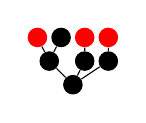
\begin{tikzpicture}[scale=.2]
\node[circle, scale=0.75, fill] (tid0) at (3,0){};
\node[circle, scale=0.75, fill] (tid1) at (1.5,1.5){};
\node[circle, scale=0.75, fill, red] (tid4) at (0.75,3){};
\node[circle, scale=0.75, fill] (tid5) at (2.25,3){};
\draw[](tid1) -- (tid4);
\draw[](tid1) -- (tid5);
\node[circle, scale=0.75, fill] (tid2) at (3.75,1.5){};
\node[circle, scale=0.75, fill, red] (tid6) at (3.75,3){};
\draw[](tid2) -- (tid6);
\node[circle, scale=0.75, fill] (tid3) at (5.25,1.5){};
\node[circle, scale=0.75, fill, red] (tid7) at (5.25,3){};
\draw[](tid3) -- (tid7);
\draw[](tid0) -- (tid1);
\draw[](tid0) -- (tid2);
\draw[](tid0) -- (tid3);

\end{tikzpicture}
\nodepart{two}
\footnotesize{4.54012}
\nodepart{three}
\footnotesize{$33\:67$}
};
\node[draw=black, rectangle split, rectangle split parts=3] (sn0x8fdea28W-12) at (-12, -48) {
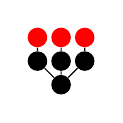
\begin{tikzpicture}[scale=.2]
\node[circle, scale=0.75, fill] (tid0) at (2.25,0){};
\node[circle, scale=0.75, fill] (tid1) at (0.75,1.5){};
\node[circle, scale=0.75, fill, red] (tid4) at (0.75,3){};
\draw[](tid1) -- (tid4);
\node[circle, scale=0.75, fill] (tid2) at (2.25,1.5){};
\node[circle, scale=0.75, fill, red] (tid5) at (2.25,3){};
\draw[](tid2) -- (tid5);
\node[circle, scale=0.75, fill] (tid3) at (3.75,1.5){};
\node[circle, scale=0.75, fill, red] (tid6) at (3.75,3){};
\draw[](tid3) -- (tid6);
\draw[](tid0) -- (tid1);
\draw[](tid0) -- (tid2);
\draw[](tid0) -- (tid3);

\end{tikzpicture}
\nodepart{two}
\footnotesize{4.21296}
\nodepart{three}
\footnotesize{$1$}
};
\node[draw=black, rectangle split, rectangle split parts=3] (sn0x8fd8170W-7) at (-7.25, -60) {
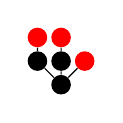
\begin{tikzpicture}[scale=.2]
\node[circle, scale=0.75, fill] (tid0) at (2.25,0){};
\node[circle, scale=0.75, fill] (tid1) at (0.75,1.5){};
\node[circle, scale=0.75, fill, red] (tid4) at (0.75,3){};
\draw[](tid1) -- (tid4);
\node[circle, scale=0.75, fill] (tid2) at (2.25,1.5){};
\node[circle, scale=0.75, fill, red] (tid5) at (2.25,3){};
\draw[](tid2) -- (tid5);
\node[circle, scale=0.75, fill, red] (tid3) at (3.75,1.5){};
\draw[](tid0) -- (tid1);
\draw[](tid0) -- (tid2);
\draw[](tid0) -- (tid3);

\end{tikzpicture}
\nodepart{two}
\footnotesize{3.87963}
\nodepart{three}
\footnotesize{$33\:67$}
};
\node[draw=black, rectangle split, rectangle split parts=3] (sn0x8fd6e28W-9) at (-9, -72) {
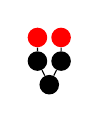
\begin{tikzpicture}[scale=.2]
\node[circle, scale=0.75, fill] (tid0) at (1.5,0){};
\node[circle, scale=0.75, fill] (tid1) at (0.75,1.5){};
\node[circle, scale=0.75, fill, red] (tid3) at (0.75,3){};
\draw[](tid1) -- (tid3);
\node[circle, scale=0.75, fill] (tid2) at (2.25,1.5){};
\node[circle, scale=0.75, fill, red] (tid4) at (2.25,3){};
\draw[](tid2) -- (tid4);
\draw[](tid0) -- (tid1);
\draw[](tid0) -- (tid2);

\end{tikzpicture}
\nodepart{two}
\footnotesize{3.75}
\nodepart{three}
\footnotesize{$1$}
};
\node[draw=black, rectangle split, rectangle split parts=3] (sn0x8fd3e80W-8) at (-8.25, -84) {
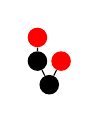
\begin{tikzpicture}[scale=.2]
\node[circle, scale=0.75, fill] (tid0) at (1.5,0){};
\node[circle, scale=0.75, fill] (tid1) at (0.75,1.5){};
\node[circle, scale=0.75, fill, red] (tid3) at (0.75,3){};
\draw[](tid1) -- (tid3);
\node[circle, scale=0.75, fill, red] (tid2) at (2.25,1.5){};
\draw[](tid0) -- (tid1);
\draw[](tid0) -- (tid2);

\end{tikzpicture}
\nodepart{two}
\footnotesize{3.25}
\nodepart{three}
\footnotesize{$50\:50$}
};
\node[draw=black, rectangle split, rectangle split parts=3] (sn0x8fd75a8W-4) at (-4.25, -96) {
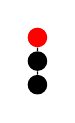
\begin{tikzpicture}[scale=.2]
\node[circle, scale=0.75, fill] (tid0) at (0.75,0){};
\node[circle, scale=0.75, fill] (tid1) at (0.75,1.5){};
\node[circle, scale=0.75, fill, red] (tid2) at (0.75,3){};
\draw[](tid1) -- (tid2);
\draw[](tid0) -- (tid1);

\end{tikzpicture}
\nodepart{two}
\footnotesize{3}
\nodepart{three}
\footnotesize{$1$}
};
\node[draw=black, rectangle split, rectangle split parts=3] (sn0x8fd30e8W-1) at (-1.75, -108) {

\begin{tikzpicture}[scale=.2]
\node[circle, scale=0.75, fill] (tid0) at (0.75,0){};
\node[circle, scale=0.75, fill, red] (tid1) at (0.75,1.5){};
\draw[](tid0) -- (tid1);

\end{tikzpicture}
\nodepart{two}
\footnotesize{2}
\nodepart{three}
\footnotesize{$1$}
};
\draw (sn0x8fd75a8W-4.south) -- (sn0x8fd30e8W-1.north);
\node[draw=black, rectangle split, rectangle split parts=3] (sn0x8fd3158W0) at (-0.75, -96) {

\begin{tikzpicture}[scale=.2]
\node[circle, scale=0.75, fill] (tid0) at (1.5,0){};
\node[circle, scale=0.75, fill, red] (tid1) at (0.75,1.5){};
\node[circle, scale=0.75, fill, red] (tid2) at (2.25,1.5){};
\draw[](tid0) -- (tid1);
\draw[](tid0) -- (tid2);

\end{tikzpicture}
\nodepart{two}
\footnotesize{2.5}
\nodepart{three}
\footnotesize{$1$}
};
\draw (sn0x8fd3158W0.south) -- (sn0x8fd30e8W-1.north);
\draw (sn0x8fd3e80W-8.south) -- (sn0x8fd75a8W-4.north);
\draw (sn0x8fd3e80W-8.south) -- (sn0x8fd3158W0.north);
\draw (sn0x8fd6e28W-9.south) -- (sn0x8fd3e80W-8.north);
\node[draw=black, rectangle split, rectangle split parts=3] (sn0x8fd4d48W-4) at (-4, -72) {
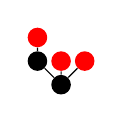
\begin{tikzpicture}[scale=.2]
\node[circle, scale=0.75, fill] (tid0) at (2.25,0){};
\node[circle, scale=0.75, fill] (tid1) at (0.75,1.5){};
\node[circle, scale=0.75, fill, red] (tid4) at (0.75,3){};
\draw[](tid1) -- (tid4);
\node[circle, scale=0.75, fill, red] (tid2) at (2.25,1.5){};
\node[circle, scale=0.75, fill, red] (tid3) at (3.75,1.5){};
\draw[](tid0) -- (tid1);
\draw[](tid0) -- (tid2);
\draw[](tid0) -- (tid3);

\end{tikzpicture}
\nodepart{two}
\footnotesize{3.44444}
\nodepart{three}
\footnotesize{$67\:33$}
};
\node[draw=black, rectangle split, rectangle split parts=3] (sn0x8fd58e8W-3) at (-3.25, -84) {
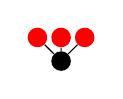
\begin{tikzpicture}[scale=.2]
\node[circle, scale=0.75, fill] (tid0) at (2.25,0){};
\node[circle, scale=0.75, fill, red] (tid1) at (0.75,1.5){};
\node[circle, scale=0.75, fill, red] (tid2) at (2.25,1.5){};
\node[circle, scale=0.75, fill, red] (tid3) at (3.75,1.5){};
\draw[](tid0) -- (tid1);
\draw[](tid0) -- (tid2);
\draw[](tid0) -- (tid3);

\end{tikzpicture}
\nodepart{two}
\footnotesize{2.83333}
\nodepart{three}
\footnotesize{$1$}
};
\draw (sn0x8fd58e8W-3.south) -- (sn0x8fd3158W0.north);
\draw (sn0x8fd4d48W-4.south) -- (sn0x8fd3e80W-8.north);
\draw (sn0x8fd4d48W-4.south) -- (sn0x8fd58e8W-3.north);
\draw (sn0x8fd8170W-7.south) -- (sn0x8fd6e28W-9.north);
\draw (sn0x8fd8170W-7.south) -- (sn0x8fd4d48W-4.north);
\draw (sn0x8fdea28W-12.south) -- (sn0x8fd8170W-7.north);
\node[draw=black, rectangle split, rectangle split parts=3] (sn0x8fd6cf8W-5) at (-5.5, -48) {
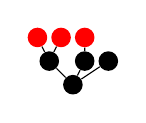
\begin{tikzpicture}[scale=.2]
\node[circle, scale=0.75, fill] (tid0) at (3,0){};
\node[circle, scale=0.75, fill] (tid1) at (1.5,1.5){};
\node[circle, scale=0.75, fill, red] (tid4) at (0.75,3){};
\node[circle, scale=0.75, fill, red] (tid5) at (2.25,3){};
\draw[](tid1) -- (tid4);
\draw[](tid1) -- (tid5);
\node[circle, scale=0.75, fill] (tid2) at (3.75,1.5){};
\node[circle, scale=0.75, fill, red] (tid6) at (3.75,3){};
\draw[](tid2) -- (tid6);
\node[circle, scale=0.75, fill] (tid3) at (5.25,1.5){};
\draw[](tid0) -- (tid1);
\draw[](tid0) -- (tid2);
\draw[](tid0) -- (tid3);

\end{tikzpicture}
\nodepart{two}
\footnotesize{4.2037}
\nodepart{three}
\footnotesize{$67\:33$}
};
\node[draw=black, rectangle split, rectangle split parts=3] (sn0x8fd6610W0) at (-0.75, -60) {
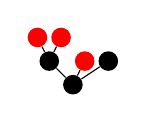
\begin{tikzpicture}[scale=.2]
\node[circle, scale=0.75, fill] (tid0) at (3,0){};
\node[circle, scale=0.75, fill] (tid1) at (1.5,1.5){};
\node[circle, scale=0.75, fill, red] (tid4) at (0.75,3){};
\node[circle, scale=0.75, fill, red] (tid5) at (2.25,3){};
\draw[](tid1) -- (tid4);
\draw[](tid1) -- (tid5);
\node[circle, scale=0.75, fill, red] (tid2) at (3.75,1.5){};
\node[circle, scale=0.75, fill] (tid3) at (5.25,1.5){};
\draw[](tid0) -- (tid1);
\draw[](tid0) -- (tid2);
\draw[](tid0) -- (tid3);

\end{tikzpicture}
\nodepart{two}
\footnotesize{3.85185}
\nodepart{three}
\footnotesize{$33\:67$}
};
\node[draw=black, rectangle split, rectangle split parts=3] (sn0x8fd7358W2) at (2.5, -72) {
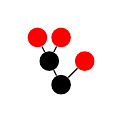
\begin{tikzpicture}[scale=.2]
\node[circle, scale=0.75, fill] (tid0) at (2.25,0){};
\node[circle, scale=0.75, fill] (tid1) at (1.5,1.5){};
\node[circle, scale=0.75, fill, red] (tid3) at (0.75,3){};
\node[circle, scale=0.75, fill, red] (tid4) at (2.25,3){};
\draw[](tid1) -- (tid3);
\draw[](tid1) -- (tid4);
\node[circle, scale=0.75, fill, red] (tid2) at (3.75,1.5){};
\draw[](tid0) -- (tid1);
\draw[](tid0) -- (tid2);

\end{tikzpicture}
\nodepart{two}
\footnotesize{3.66667}
\nodepart{three}
\footnotesize{$33\:67$}
};
\node[draw=black, rectangle split, rectangle split parts=3] (sn0x8fd8a08W3) at (3.25, -84) {
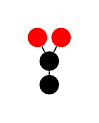
\begin{tikzpicture}[scale=.2]
\node[circle, scale=0.75, fill] (tid0) at (1.5,0){};
\node[circle, scale=0.75, fill] (tid1) at (1.5,1.5){};
\node[circle, scale=0.75, fill, red] (tid2) at (0.75,3){};
\node[circle, scale=0.75, fill, red] (tid3) at (2.25,3){};
\draw[](tid1) -- (tid2);
\draw[](tid1) -- (tid3);
\draw[](tid0) -- (tid1);

\end{tikzpicture}
\nodepart{two}
\footnotesize{3.5}
\nodepart{three}
\footnotesize{$1$}
};
\draw (sn0x8fd8a08W3.south) -- (sn0x8fd75a8W-4.north);
\draw (sn0x8fd7358W2.south) -- (sn0x8fd8a08W3.north);
\draw (sn0x8fd7358W2.south) -- (sn0x8fd3e80W-8.north);
\draw (sn0x8fd6610W0.south) -- (sn0x8fd7358W2.north);
\draw (sn0x8fd6610W0.south) -- (sn0x8fd4d48W-4.north);
\draw (sn0x8fd6cf8W-5.south) -- (sn0x8fd8170W-7.north);
\draw (sn0x8fd6cf8W-5.south) -- (sn0x8fd6610W0.north);
\draw (sn0x8fd3d30W-22.south) -- (sn0x8fdea28W-12.north);
\draw (sn0x8fd3d30W-22.south) -- (sn0x8fd6cf8W-5.north);
\node[draw=black, rectangle split, rectangle split parts=3] (sn0x8fde270W-14) at (-14.25, -36) {
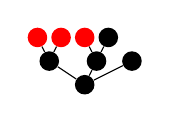
\begin{tikzpicture}[scale=.2]
\node[circle, scale=0.75, fill] (tid0) at (3.75,0){};
\node[circle, scale=0.75, fill] (tid1) at (1.5,1.5){};
\node[circle, scale=0.75, fill, red] (tid4) at (0.75,3){};
\node[circle, scale=0.75, fill, red] (tid5) at (2.25,3){};
\draw[](tid1) -- (tid4);
\draw[](tid1) -- (tid5);
\node[circle, scale=0.75, fill] (tid2) at (4.5,1.5){};
\node[circle, scale=0.75, fill, red] (tid6) at (3.75,3){};
\node[circle, scale=0.75, fill] (tid7) at (5.25,3){};
\draw[](tid2) -- (tid6);
\draw[](tid2) -- (tid7);
\node[circle, scale=0.75, fill] (tid3) at (6.75,1.5){};
\draw[](tid0) -- (tid1);
\draw[](tid0) -- (tid2);
\draw[](tid0) -- (tid3);

\end{tikzpicture}
\nodepart{two}
\footnotesize{4.53704}
\nodepart{three}
\footnotesize{$1$}
};
\draw (sn0x8fde270W-14.south) -- (sn0x8fd6cf8W-5.north);
\draw (sn0x8fd3f88W-20.south) -- (sn0x8fd3d30W-22.north);
\draw (sn0x8fd3f88W-20.south) -- (sn0x8fde270W-14.north);
\node[draw=black, rectangle split, rectangle split parts=3] (sn0x8fd3e00W-11) at (-11, -24) {
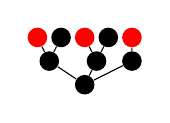
\begin{tikzpicture}[scale=.2]
\node[circle, scale=0.75, fill] (tid0) at (3.75,0){};
\node[circle, scale=0.75, fill] (tid1) at (1.5,1.5){};
\node[circle, scale=0.75, fill, red] (tid4) at (0.75,3){};
\node[circle, scale=0.75, fill] (tid5) at (2.25,3){};
\draw[](tid1) -- (tid4);
\draw[](tid1) -- (tid5);
\node[circle, scale=0.75, fill] (tid2) at (4.5,1.5){};
\node[circle, scale=0.75, fill, red] (tid6) at (3.75,3){};
\node[circle, scale=0.75, fill] (tid7) at (5.25,3){};
\draw[](tid2) -- (tid6);
\draw[](tid2) -- (tid7);
\node[circle, scale=0.75, fill] (tid3) at (6.75,1.5){};
\node[circle, scale=0.75, fill, red] (tid8) at (6.75,3){};
\draw[](tid3) -- (tid8);
\draw[](tid0) -- (tid1);
\draw[](tid0) -- (tid2);
\draw[](tid0) -- (tid3);

\end{tikzpicture}
\nodepart{two}
\footnotesize{4.87346}
\nodepart{three}
\footnotesize{$33\:33\:33$}
};
\node[draw=black, rectangle split, rectangle split parts=3] (sn0x8fd4e10W-4) at (-4.75, -36) {
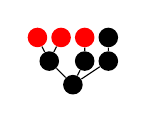
\begin{tikzpicture}[scale=.2]
\node[circle, scale=0.75, fill] (tid0) at (3,0){};
\node[circle, scale=0.75, fill] (tid1) at (1.5,1.5){};
\node[circle, scale=0.75, fill, red] (tid4) at (0.75,3){};
\node[circle, scale=0.75, fill, red] (tid5) at (2.25,3){};
\draw[](tid1) -- (tid4);
\draw[](tid1) -- (tid5);
\node[circle, scale=0.75, fill] (tid2) at (3.75,1.5){};
\node[circle, scale=0.75, fill, red] (tid6) at (3.75,3){};
\draw[](tid2) -- (tid6);
\node[circle, scale=0.75, fill] (tid3) at (5.25,1.5){};
\node[circle, scale=0.75, fill] (tid7) at (5.25,3){};
\draw[](tid3) -- (tid7);
\draw[](tid0) -- (tid1);
\draw[](tid0) -- (tid2);
\draw[](tid0) -- (tid3);

\end{tikzpicture}
\nodepart{two}
\footnotesize{4.54321}
\nodepart{three}
\footnotesize{$67\:33$}
};
\draw (sn0x8fd4e10W-4.south) -- (sn0x8fdea28W-12.north);
\draw (sn0x8fd4e10W-4.south) -- (sn0x8fd6cf8W-5.north);
\draw (sn0x8fd3e00W-11.south) -- (sn0x8fd3d30W-22.north);
\draw (sn0x8fd3e00W-11.south) -- (sn0x8fd4e10W-4.north);
\draw (sn0x8fd3e00W-11.south) -- (sn0x8fde270W-14.north);
\node[draw=black, rectangle split, rectangle split parts=3] (sn0x8fde428W-1) at (-1.5, -24) {
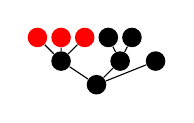
\begin{tikzpicture}[scale=.2]
\node[circle, scale=0.75, fill] (tid0) at (4.5,0){};
\node[circle, scale=0.75, fill] (tid1) at (2.25,1.5){};
\node[circle, scale=0.75, fill, red] (tid4) at (0.75,3){};
\node[circle, scale=0.75, fill, red] (tid5) at (2.25,3){};
\node[circle, scale=0.75, fill, red] (tid6) at (3.75,3){};
\draw[](tid1) -- (tid4);
\draw[](tid1) -- (tid5);
\draw[](tid1) -- (tid6);
\node[circle, scale=0.75, fill] (tid2) at (6,1.5){};
\node[circle, scale=0.75, fill] (tid7) at (5.25,3){};
\node[circle, scale=0.75, fill] (tid8) at (6.75,3){};
\draw[](tid2) -- (tid7);
\draw[](tid2) -- (tid8);
\node[circle, scale=0.75, fill] (tid3) at (8.25,1.5){};
\draw[](tid0) -- (tid1);
\draw[](tid0) -- (tid2);
\draw[](tid0) -- (tid3);

\end{tikzpicture}
\nodepart{two}
\footnotesize{4.87037}
\nodepart{three}
\footnotesize{$1$}
};
\draw (sn0x8fde428W-1.south) -- (sn0x8fde270W-14.north);
\node[draw=black, rectangle split, rectangle split parts=3] (sn0x8fd34c8W9) at (9.5, -24) {
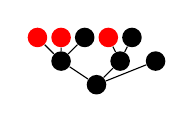
\begin{tikzpicture}[scale=.2]
\node[circle, scale=0.75, fill] (tid0) at (4.5,0){};
\node[circle, scale=0.75, fill] (tid1) at (2.25,1.5){};
\node[circle, scale=0.75, fill, red] (tid4) at (0.75,3){};
\node[circle, scale=0.75, fill, red] (tid5) at (2.25,3){};
\node[circle, scale=0.75, fill] (tid6) at (3.75,3){};
\draw[](tid1) -- (tid4);
\draw[](tid1) -- (tid5);
\draw[](tid1) -- (tid6);
\node[circle, scale=0.75, fill] (tid2) at (6,1.5){};
\node[circle, scale=0.75, fill, red] (tid7) at (5.25,3){};
\node[circle, scale=0.75, fill] (tid8) at (6.75,3){};
\draw[](tid2) -- (tid7);
\draw[](tid2) -- (tid8);
\node[circle, scale=0.75, fill] (tid3) at (8.25,1.5){};
\draw[](tid0) -- (tid1);
\draw[](tid0) -- (tid2);
\draw[](tid0) -- (tid3);

\end{tikzpicture}
\nodepart{two}
\footnotesize{4.86934}
\nodepart{three}
\footnotesize{$67\:17\:17$}
};
\node[draw=black, rectangle split, rectangle split parts=3] (sn0x8fdefe0W3) at (3.25, -36) {
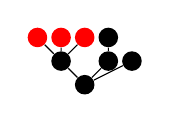
\begin{tikzpicture}[scale=.2]
\node[circle, scale=0.75, fill] (tid0) at (3.75,0){};
\node[circle, scale=0.75, fill] (tid1) at (2.25,1.5){};
\node[circle, scale=0.75, fill, red] (tid4) at (0.75,3){};
\node[circle, scale=0.75, fill, red] (tid5) at (2.25,3){};
\node[circle, scale=0.75, fill, red] (tid6) at (3.75,3){};
\draw[](tid1) -- (tid4);
\draw[](tid1) -- (tid5);
\draw[](tid1) -- (tid6);
\node[circle, scale=0.75, fill] (tid2) at (5.25,1.5){};
\node[circle, scale=0.75, fill] (tid7) at (5.25,3){};
\draw[](tid2) -- (tid7);
\node[circle, scale=0.75, fill] (tid3) at (6.75,1.5){};
\draw[](tid0) -- (tid1);
\draw[](tid0) -- (tid2);
\draw[](tid0) -- (tid3);

\end{tikzpicture}
\nodepart{two}
\footnotesize{4.53704}
\nodepart{three}
\footnotesize{$1$}
};
\draw (sn0x8fdefe0W3.south) -- (sn0x8fd6cf8W-5.north);
\node[draw=black, rectangle split, rectangle split parts=3] (sn0x8fde610W12) at (12.75, -36) {
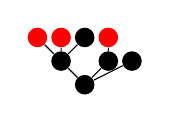
\begin{tikzpicture}[scale=.2]
\node[circle, scale=0.75, fill] (tid0) at (3.75,0){};
\node[circle, scale=0.75, fill] (tid1) at (2.25,1.5){};
\node[circle, scale=0.75, fill, red] (tid4) at (0.75,3){};
\node[circle, scale=0.75, fill, red] (tid5) at (2.25,3){};
\node[circle, scale=0.75, fill] (tid6) at (3.75,3){};
\draw[](tid1) -- (tid4);
\draw[](tid1) -- (tid5);
\draw[](tid1) -- (tid6);
\node[circle, scale=0.75, fill] (tid2) at (5.25,1.5){};
\node[circle, scale=0.75, fill, red] (tid7) at (5.25,3){};
\draw[](tid2) -- (tid7);
\node[circle, scale=0.75, fill] (tid3) at (6.75,1.5){};
\draw[](tid0) -- (tid1);
\draw[](tid0) -- (tid2);
\draw[](tid0) -- (tid3);

\end{tikzpicture}
\nodepart{two}
\footnotesize{4.53086}
\nodepart{three}
\footnotesize{$67\:33$}
};
\node[draw=black, rectangle split, rectangle split parts=3] (sn0x8fdf3d0W2) at (2.5, -48) {
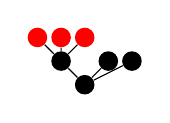
\begin{tikzpicture}[scale=.2]
\node[circle, scale=0.75, fill] (tid0) at (3.75,0){};
\node[circle, scale=0.75, fill] (tid1) at (2.25,1.5){};
\node[circle, scale=0.75, fill, red] (tid4) at (0.75,3){};
\node[circle, scale=0.75, fill, red] (tid5) at (2.25,3){};
\node[circle, scale=0.75, fill, red] (tid6) at (3.75,3){};
\draw[](tid1) -- (tid4);
\draw[](tid1) -- (tid5);
\draw[](tid1) -- (tid6);
\node[circle, scale=0.75, fill] (tid2) at (5.25,1.5){};
\node[circle, scale=0.75, fill] (tid3) at (6.75,1.5){};
\draw[](tid0) -- (tid1);
\draw[](tid0) -- (tid2);
\draw[](tid0) -- (tid3);

\end{tikzpicture}
\nodepart{two}
\footnotesize{4.18519}
\nodepart{three}
\footnotesize{$1$}
};
\draw (sn0x8fdf3d0W2.south) -- (sn0x8fd6610W0.north);
\draw (sn0x8fde610W12.south) -- (sn0x8fd6cf8W-5.north);
\draw (sn0x8fde610W12.south) -- (sn0x8fdf3d0W2.north);
\draw (sn0x8fd34c8W9.south) -- (sn0x8fde270W-14.north);
\draw (sn0x8fd34c8W9.south) -- (sn0x8fdefe0W3.north);
\draw (sn0x8fd34c8W9.south) -- (sn0x8fde610W12.north);
\draw (sn0x8fd4380W-5.south) -- (sn0x8fd3f88W-20.north);
\draw (sn0x8fd4380W-5.south) -- (sn0x8fd3e00W-11.north);
\draw (sn0x8fd4380W-5.south) -- (sn0x8fde428W-1.north);
\draw (sn0x8fd4380W-5.south) -- (sn0x8fd34c8W9.north);
\end{tikzpicture}

%%% Local Variables:
%%% TeX-master: "thesis/thesis.tex"
%%% End: 

\begin{tikzpicture}[scale=.2, anchor=south west]
\node[draw=black, rectangle split, rectangle split parts=3] (sn0x8fd43e0W-5) at (-5.5, -12) {
\begin{tikzpicture}[scale=.2]
\node[circle, scale=0.75, fill] (tid0) at (4.5,0){};
\node[circle, scale=0.75, fill] (tid1) at (2.25,1.5){};
\node[circle, scale=0.75, fill, red] (tid4) at (0.75,3){};
\node[circle, scale=0.75, fill, red] (tid5) at (2.25,3){};
\node[circle, scale=0.75, fill, red] (tid6) at (3.75,3){};
\draw[](tid1) -- (tid4);
\draw[](tid1) -- (tid5);
\draw[](tid1) -- (tid6);
\node[circle, scale=0.75, fill] (tid2) at (6,1.5){};
\node[circle, scale=0.75, fill] (tid7) at (5.25,3){};
\node[circle, scale=0.75, fill] (tid8) at (6.75,3){};
\draw[](tid2) -- (tid7);
\draw[](tid2) -- (tid8);
\node[circle, scale=0.75, fill] (tid3) at (8.25,1.5){};
\node[circle, scale=0.75, fill] (tid9) at (8.25,3){};
\draw[](tid3) -- (tid9);
\draw[](tid0) -- (tid1);
\draw[](tid0) -- (tid2);
\draw[](tid0) -- (tid3);

\end{tikzpicture}
\nodepart{two}
\footnotesize{5.20782}
\nodepart{three}
\footnotesize{$67\:33$}
};
\node[draw=black, rectangle split, rectangle split parts=3] (sn0x8fdf1c8W-9) at (-9.5, -24) {
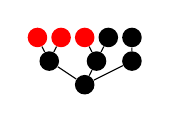
\begin{tikzpicture}[scale=.2]
\node[circle, scale=0.75, fill] (tid0) at (3.75,0){};
\node[circle, scale=0.75, fill] (tid1) at (1.5,1.5){};
\node[circle, scale=0.75, fill, red] (tid4) at (0.75,3){};
\node[circle, scale=0.75, fill, red] (tid5) at (2.25,3){};
\draw[](tid1) -- (tid4);
\draw[](tid1) -- (tid5);
\node[circle, scale=0.75, fill] (tid2) at (4.5,1.5){};
\node[circle, scale=0.75, fill, red] (tid6) at (3.75,3){};
\node[circle, scale=0.75, fill] (tid7) at (5.25,3){};
\draw[](tid2) -- (tid6);
\draw[](tid2) -- (tid7);
\node[circle, scale=0.75, fill] (tid3) at (6.75,1.5){};
\node[circle, scale=0.75, fill] (tid8) at (6.75,3){};
\draw[](tid3) -- (tid8);
\draw[](tid0) -- (tid1);
\draw[](tid0) -- (tid2);
\draw[](tid0) -- (tid3);

\end{tikzpicture}
\nodepart{two}
\footnotesize{4.87551}
\nodepart{three}
\footnotesize{$67\:33$}
};
\node[draw=black, rectangle split, rectangle split parts=3] (sn0x8fd4e10W-12) at (-12.75, -36) {
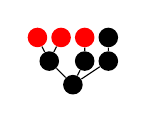
\begin{tikzpicture}[scale=.2]
\node[circle, scale=0.75, fill] (tid0) at (3,0){};
\node[circle, scale=0.75, fill] (tid1) at (1.5,1.5){};
\node[circle, scale=0.75, fill, red] (tid4) at (0.75,3){};
\node[circle, scale=0.75, fill, red] (tid5) at (2.25,3){};
\draw[](tid1) -- (tid4);
\draw[](tid1) -- (tid5);
\node[circle, scale=0.75, fill] (tid2) at (3.75,1.5){};
\node[circle, scale=0.75, fill, red] (tid6) at (3.75,3){};
\draw[](tid2) -- (tid6);
\node[circle, scale=0.75, fill] (tid3) at (5.25,1.5){};
\node[circle, scale=0.75, fill] (tid7) at (5.25,3){};
\draw[](tid3) -- (tid7);
\draw[](tid0) -- (tid1);
\draw[](tid0) -- (tid2);
\draw[](tid0) -- (tid3);

\end{tikzpicture}
\nodepart{two}
\footnotesize{4.54321}
\nodepart{three}
\footnotesize{$67\:33$}
};
\node[draw=black, rectangle split, rectangle split parts=3] (sn0x8fdea28W-7) at (-7.25, -48) {
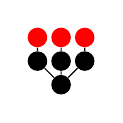
\begin{tikzpicture}[scale=.2]
\node[circle, scale=0.75, fill] (tid0) at (2.25,0){};
\node[circle, scale=0.75, fill] (tid1) at (0.75,1.5){};
\node[circle, scale=0.75, fill, red] (tid4) at (0.75,3){};
\draw[](tid1) -- (tid4);
\node[circle, scale=0.75, fill] (tid2) at (2.25,1.5){};
\node[circle, scale=0.75, fill, red] (tid5) at (2.25,3){};
\draw[](tid2) -- (tid5);
\node[circle, scale=0.75, fill] (tid3) at (3.75,1.5){};
\node[circle, scale=0.75, fill, red] (tid6) at (3.75,3){};
\draw[](tid3) -- (tid6);
\draw[](tid0) -- (tid1);
\draw[](tid0) -- (tid2);
\draw[](tid0) -- (tid3);

\end{tikzpicture}
\nodepart{two}
\footnotesize{4.21296}
\nodepart{three}
\footnotesize{$1$}
};
\node[draw=black, rectangle split, rectangle split parts=3] (sn0x8fd8170W-7) at (-7.25, -60) {
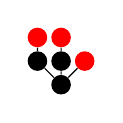
\begin{tikzpicture}[scale=.2]
\node[circle, scale=0.75, fill] (tid0) at (2.25,0){};
\node[circle, scale=0.75, fill] (tid1) at (0.75,1.5){};
\node[circle, scale=0.75, fill, red] (tid4) at (0.75,3){};
\draw[](tid1) -- (tid4);
\node[circle, scale=0.75, fill] (tid2) at (2.25,1.5){};
\node[circle, scale=0.75, fill, red] (tid5) at (2.25,3){};
\draw[](tid2) -- (tid5);
\node[circle, scale=0.75, fill, red] (tid3) at (3.75,1.5){};
\draw[](tid0) -- (tid1);
\draw[](tid0) -- (tid2);
\draw[](tid0) -- (tid3);

\end{tikzpicture}
\nodepart{two}
\footnotesize{3.87963}
\nodepart{three}
\footnotesize{$33\:67$}
};
\node[draw=black, rectangle split, rectangle split parts=3] (sn0x8fd6e28W-9) at (-9, -72) {
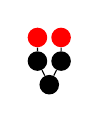
\begin{tikzpicture}[scale=.2]
\node[circle, scale=0.75, fill] (tid0) at (1.5,0){};
\node[circle, scale=0.75, fill] (tid1) at (0.75,1.5){};
\node[circle, scale=0.75, fill, red] (tid3) at (0.75,3){};
\draw[](tid1) -- (tid3);
\node[circle, scale=0.75, fill] (tid2) at (2.25,1.5){};
\node[circle, scale=0.75, fill, red] (tid4) at (2.25,3){};
\draw[](tid2) -- (tid4);
\draw[](tid0) -- (tid1);
\draw[](tid0) -- (tid2);

\end{tikzpicture}
\nodepart{two}
\footnotesize{3.75}
\nodepart{three}
\footnotesize{$1$}
};
\node[draw=black, rectangle split, rectangle split parts=3] (sn0x8fd3e80W-8) at (-8.25, -84) {
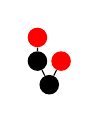
\begin{tikzpicture}[scale=.2]
\node[circle, scale=0.75, fill] (tid0) at (1.5,0){};
\node[circle, scale=0.75, fill] (tid1) at (0.75,1.5){};
\node[circle, scale=0.75, fill, red] (tid3) at (0.75,3){};
\draw[](tid1) -- (tid3);
\node[circle, scale=0.75, fill, red] (tid2) at (2.25,1.5){};
\draw[](tid0) -- (tid1);
\draw[](tid0) -- (tid2);

\end{tikzpicture}
\nodepart{two}
\footnotesize{3.25}
\nodepart{three}
\footnotesize{$50\:50$}
};
\node[draw=black, rectangle split, rectangle split parts=3] (sn0x8fd75a8W-4) at (-4.25, -96) {
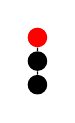
\begin{tikzpicture}[scale=.2]
\node[circle, scale=0.75, fill] (tid0) at (0.75,0){};
\node[circle, scale=0.75, fill] (tid1) at (0.75,1.5){};
\node[circle, scale=0.75, fill, red] (tid2) at (0.75,3){};
\draw[](tid1) -- (tid2);
\draw[](tid0) -- (tid1);

\end{tikzpicture}
\nodepart{two}
\footnotesize{3}
\nodepart{three}
\footnotesize{$1$}
};
\node[draw=black, rectangle split, rectangle split parts=3] (sn0x8fd30e8W-1) at (-1.75, -108) {

\begin{tikzpicture}[scale=.2]
\node[circle, scale=0.75, fill] (tid0) at (0.75,0){};
\node[circle, scale=0.75, fill, red] (tid1) at (0.75,1.5){};
\draw[](tid0) -- (tid1);

\end{tikzpicture}
\nodepart{two}
\footnotesize{2}
\nodepart{three}
\footnotesize{$1$}
};
\draw (sn0x8fd75a8W-4.south) -- (sn0x8fd30e8W-1.north);
\node[draw=black, rectangle split, rectangle split parts=3] (sn0x8fd3158W0) at (-0.75, -96) {

\begin{tikzpicture}[scale=.2]
\node[circle, scale=0.75, fill] (tid0) at (1.5,0){};
\node[circle, scale=0.75, fill, red] (tid1) at (0.75,1.5){};
\node[circle, scale=0.75, fill, red] (tid2) at (2.25,1.5){};
\draw[](tid0) -- (tid1);
\draw[](tid0) -- (tid2);

\end{tikzpicture}
\nodepart{two}
\footnotesize{2.5}
\nodepart{three}
\footnotesize{$1$}
};
\draw (sn0x8fd3158W0.south) -- (sn0x8fd30e8W-1.north);
\draw (sn0x8fd3e80W-8.south) -- (sn0x8fd75a8W-4.north);
\draw (sn0x8fd3e80W-8.south) -- (sn0x8fd3158W0.north);
\draw (sn0x8fd6e28W-9.south) -- (sn0x8fd3e80W-8.north);
\node[draw=black, rectangle split, rectangle split parts=3] (sn0x8fd4d48W-4) at (-4, -72) {
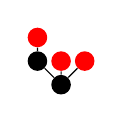
\begin{tikzpicture}[scale=.2]
\node[circle, scale=0.75, fill] (tid0) at (2.25,0){};
\node[circle, scale=0.75, fill] (tid1) at (0.75,1.5){};
\node[circle, scale=0.75, fill, red] (tid4) at (0.75,3){};
\draw[](tid1) -- (tid4);
\node[circle, scale=0.75, fill, red] (tid2) at (2.25,1.5){};
\node[circle, scale=0.75, fill, red] (tid3) at (3.75,1.5){};
\draw[](tid0) -- (tid1);
\draw[](tid0) -- (tid2);
\draw[](tid0) -- (tid3);

\end{tikzpicture}
\nodepart{two}
\footnotesize{3.44444}
\nodepart{three}
\footnotesize{$67\:33$}
};
\node[draw=black, rectangle split, rectangle split parts=3] (sn0x8fd58e8W-3) at (-3.25, -84) {
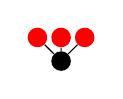
\begin{tikzpicture}[scale=.2]
\node[circle, scale=0.75, fill] (tid0) at (2.25,0){};
\node[circle, scale=0.75, fill, red] (tid1) at (0.75,1.5){};
\node[circle, scale=0.75, fill, red] (tid2) at (2.25,1.5){};
\node[circle, scale=0.75, fill, red] (tid3) at (3.75,1.5){};
\draw[](tid0) -- (tid1);
\draw[](tid0) -- (tid2);
\draw[](tid0) -- (tid3);

\end{tikzpicture}
\nodepart{two}
\footnotesize{2.83333}
\nodepart{three}
\footnotesize{$1$}
};
\draw (sn0x8fd58e8W-3.south) -- (sn0x8fd3158W0.north);
\draw (sn0x8fd4d48W-4.south) -- (sn0x8fd3e80W-8.north);
\draw (sn0x8fd4d48W-4.south) -- (sn0x8fd58e8W-3.north);
\draw (sn0x8fd8170W-7.south) -- (sn0x8fd6e28W-9.north);
\draw (sn0x8fd8170W-7.south) -- (sn0x8fd4d48W-4.north);
\draw (sn0x8fdea28W-7.south) -- (sn0x8fd8170W-7.north);
\node[draw=black, rectangle split, rectangle split parts=3] (sn0x8fd6cf8W0) at (-0.75, -48) {
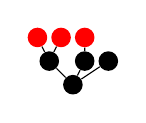
\begin{tikzpicture}[scale=.2]
\node[circle, scale=0.75, fill] (tid0) at (3,0){};
\node[circle, scale=0.75, fill] (tid1) at (1.5,1.5){};
\node[circle, scale=0.75, fill, red] (tid4) at (0.75,3){};
\node[circle, scale=0.75, fill, red] (tid5) at (2.25,3){};
\draw[](tid1) -- (tid4);
\draw[](tid1) -- (tid5);
\node[circle, scale=0.75, fill] (tid2) at (3.75,1.5){};
\node[circle, scale=0.75, fill, red] (tid6) at (3.75,3){};
\draw[](tid2) -- (tid6);
\node[circle, scale=0.75, fill] (tid3) at (5.25,1.5){};
\draw[](tid0) -- (tid1);
\draw[](tid0) -- (tid2);
\draw[](tid0) -- (tid3);

\end{tikzpicture}
\nodepart{two}
\footnotesize{4.2037}
\nodepart{three}
\footnotesize{$67\:33$}
};
\node[draw=black, rectangle split, rectangle split parts=3] (sn0x8fd6610W0) at (-0.75, -60) {
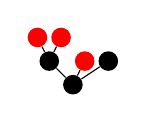
\begin{tikzpicture}[scale=.2]
\node[circle, scale=0.75, fill] (tid0) at (3,0){};
\node[circle, scale=0.75, fill] (tid1) at (1.5,1.5){};
\node[circle, scale=0.75, fill, red] (tid4) at (0.75,3){};
\node[circle, scale=0.75, fill, red] (tid5) at (2.25,3){};
\draw[](tid1) -- (tid4);
\draw[](tid1) -- (tid5);
\node[circle, scale=0.75, fill, red] (tid2) at (3.75,1.5){};
\node[circle, scale=0.75, fill] (tid3) at (5.25,1.5){};
\draw[](tid0) -- (tid1);
\draw[](tid0) -- (tid2);
\draw[](tid0) -- (tid3);

\end{tikzpicture}
\nodepart{two}
\footnotesize{3.85185}
\nodepart{three}
\footnotesize{$33\:67$}
};
\node[draw=black, rectangle split, rectangle split parts=3] (sn0x8fd7358W2) at (2.5, -72) {
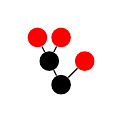
\begin{tikzpicture}[scale=.2]
\node[circle, scale=0.75, fill] (tid0) at (2.25,0){};
\node[circle, scale=0.75, fill] (tid1) at (1.5,1.5){};
\node[circle, scale=0.75, fill, red] (tid3) at (0.75,3){};
\node[circle, scale=0.75, fill, red] (tid4) at (2.25,3){};
\draw[](tid1) -- (tid3);
\draw[](tid1) -- (tid4);
\node[circle, scale=0.75, fill, red] (tid2) at (3.75,1.5){};
\draw[](tid0) -- (tid1);
\draw[](tid0) -- (tid2);

\end{tikzpicture}
\nodepart{two}
\footnotesize{3.66667}
\nodepart{three}
\footnotesize{$33\:67$}
};
\node[draw=black, rectangle split, rectangle split parts=3] (sn0x8fd8a08W3) at (3.25, -84) {
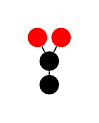
\begin{tikzpicture}[scale=.2]
\node[circle, scale=0.75, fill] (tid0) at (1.5,0){};
\node[circle, scale=0.75, fill] (tid1) at (1.5,1.5){};
\node[circle, scale=0.75, fill, red] (tid2) at (0.75,3){};
\node[circle, scale=0.75, fill, red] (tid3) at (2.25,3){};
\draw[](tid1) -- (tid2);
\draw[](tid1) -- (tid3);
\draw[](tid0) -- (tid1);

\end{tikzpicture}
\nodepart{two}
\footnotesize{3.5}
\nodepart{three}
\footnotesize{$1$}
};
\draw (sn0x8fd8a08W3.south) -- (sn0x8fd75a8W-4.north);
\draw (sn0x8fd7358W2.south) -- (sn0x8fd8a08W3.north);
\draw (sn0x8fd7358W2.south) -- (sn0x8fd3e80W-8.north);
\draw (sn0x8fd6610W0.south) -- (sn0x8fd7358W2.north);
\draw (sn0x8fd6610W0.south) -- (sn0x8fd4d48W-4.north);
\draw (sn0x8fd6cf8W0.south) -- (sn0x8fd8170W-7.north);
\draw (sn0x8fd6cf8W0.south) -- (sn0x8fd6610W0.north);
\draw (sn0x8fd4e10W-12.south) -- (sn0x8fdea28W-7.north);
\draw (sn0x8fd4e10W-12.south) -- (sn0x8fd6cf8W0.north);
\node[draw=black, rectangle split, rectangle split parts=3] (sn0x8fd3d30W-4) at (-4.75, -36) {
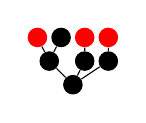
\begin{tikzpicture}[scale=.2]
\node[circle, scale=0.75, fill] (tid0) at (3,0){};
\node[circle, scale=0.75, fill] (tid1) at (1.5,1.5){};
\node[circle, scale=0.75, fill, red] (tid4) at (0.75,3){};
\node[circle, scale=0.75, fill] (tid5) at (2.25,3){};
\draw[](tid1) -- (tid4);
\draw[](tid1) -- (tid5);
\node[circle, scale=0.75, fill] (tid2) at (3.75,1.5){};
\node[circle, scale=0.75, fill, red] (tid6) at (3.75,3){};
\draw[](tid2) -- (tid6);
\node[circle, scale=0.75, fill] (tid3) at (5.25,1.5){};
\node[circle, scale=0.75, fill, red] (tid7) at (5.25,3){};
\draw[](tid3) -- (tid7);
\draw[](tid0) -- (tid1);
\draw[](tid0) -- (tid2);
\draw[](tid0) -- (tid3);

\end{tikzpicture}
\nodepart{two}
\footnotesize{4.54012}
\nodepart{three}
\footnotesize{$33\:67$}
};
\draw (sn0x8fd3d30W-4.south) -- (sn0x8fdea28W-7.north);
\draw (sn0x8fd3d30W-4.south) -- (sn0x8fd6cf8W0.north);
\draw (sn0x8fdf1c8W-9.south) -- (sn0x8fd4e10W-12.north);
\draw (sn0x8fdf1c8W-9.south) -- (sn0x8fd3d30W-4.north);
\node[draw=black, rectangle split, rectangle split parts=3] (sn0x8fd3f88W0) at (0, -24) {
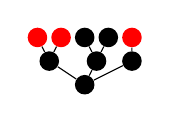
\begin{tikzpicture}[scale=.2]
\node[circle, scale=0.75, fill] (tid0) at (3.75,0){};
\node[circle, scale=0.75, fill] (tid1) at (1.5,1.5){};
\node[circle, scale=0.75, fill, red] (tid4) at (0.75,3){};
\node[circle, scale=0.75, fill, red] (tid5) at (2.25,3){};
\draw[](tid1) -- (tid4);
\draw[](tid1) -- (tid5);
\node[circle, scale=0.75, fill] (tid2) at (4.5,1.5){};
\node[circle, scale=0.75, fill] (tid6) at (3.75,3){};
\node[circle, scale=0.75, fill] (tid7) at (5.25,3){};
\draw[](tid2) -- (tid6);
\draw[](tid2) -- (tid7);
\node[circle, scale=0.75, fill] (tid3) at (6.75,1.5){};
\node[circle, scale=0.75, fill, red] (tid8) at (6.75,3){};
\draw[](tid3) -- (tid8);
\draw[](tid0) -- (tid1);
\draw[](tid0) -- (tid2);
\draw[](tid0) -- (tid3);

\end{tikzpicture}
\nodepart{two}
\footnotesize{4.87243}
\nodepart{three}
\footnotesize{$67\:33$}
};
\node[draw=black, rectangle split, rectangle split parts=3] (sn0x8fde270W3) at (3.25, -36) {
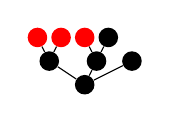
\begin{tikzpicture}[scale=.2]
\node[circle, scale=0.75, fill] (tid0) at (3.75,0){};
\node[circle, scale=0.75, fill] (tid1) at (1.5,1.5){};
\node[circle, scale=0.75, fill, red] (tid4) at (0.75,3){};
\node[circle, scale=0.75, fill, red] (tid5) at (2.25,3){};
\draw[](tid1) -- (tid4);
\draw[](tid1) -- (tid5);
\node[circle, scale=0.75, fill] (tid2) at (4.5,1.5){};
\node[circle, scale=0.75, fill, red] (tid6) at (3.75,3){};
\node[circle, scale=0.75, fill] (tid7) at (5.25,3){};
\draw[](tid2) -- (tid6);
\draw[](tid2) -- (tid7);
\node[circle, scale=0.75, fill] (tid3) at (6.75,1.5){};
\draw[](tid0) -- (tid1);
\draw[](tid0) -- (tid2);
\draw[](tid0) -- (tid3);

\end{tikzpicture}
\nodepart{two}
\footnotesize{4.53704}
\nodepart{three}
\footnotesize{$1$}
};
\draw (sn0x8fde270W3.south) -- (sn0x8fd6cf8W0.north);
\draw (sn0x8fd3f88W0.south) -- (sn0x8fd3d30W-4.north);
\draw (sn0x8fd3f88W0.south) -- (sn0x8fde270W3.north);
\draw (sn0x8fd43e0W-5.south) -- (sn0x8fdf1c8W-9.north);
\draw (sn0x8fd43e0W-5.south) -- (sn0x8fd3f88W0.north);
\end{tikzpicture}

%%% Local Variables:
%%% TeX-master: "thesis/thesis.tex"
%%% End: 

\begin{tikzpicture}[scale=.2, anchor=south west]
\node[draw=black, rectangle split, rectangle split parts=3] (sn0x8fd4440W-5) at (-5.5, -12) {
\begin{tikzpicture}[scale=.2]
\node[circle, scale=0.75, fill] (tid0) at (4.5,0){};
\node[circle, scale=0.75, fill] (tid1) at (2.25,1.5){};
\node[circle, scale=0.75, fill, red] (tid4) at (0.75,3){};
\node[circle, scale=0.75, fill, red] (tid5) at (2.25,3){};
\node[circle, scale=0.75, fill] (tid6) at (3.75,3){};
\draw[](tid1) -- (tid4);
\draw[](tid1) -- (tid5);
\draw[](tid1) -- (tid6);
\node[circle, scale=0.75, fill] (tid2) at (6,1.5){};
\node[circle, scale=0.75, fill, red] (tid7) at (5.25,3){};
\node[circle, scale=0.75, fill] (tid8) at (6.75,3){};
\draw[](tid2) -- (tid7);
\draw[](tid2) -- (tid8);
\node[circle, scale=0.75, fill] (tid3) at (8.25,1.5){};
\node[circle, scale=0.75, fill] (tid9) at (8.25,3){};
\draw[](tid3) -- (tid9);
\draw[](tid0) -- (tid1);
\draw[](tid0) -- (tid2);
\draw[](tid0) -- (tid3);

\end{tikzpicture}
\nodepart{two}
\footnotesize{5.20782}
\nodepart{three}
\footnotesize{$44\:22\:11\:22$}
};
\node[draw=black, rectangle split, rectangle split parts=3] (sn0x8fdf1c8W-19) at (-19, -24) {
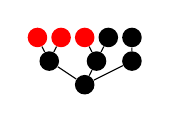
\begin{tikzpicture}[scale=.2]
\node[circle, scale=0.75, fill] (tid0) at (3.75,0){};
\node[circle, scale=0.75, fill] (tid1) at (1.5,1.5){};
\node[circle, scale=0.75, fill, red] (tid4) at (0.75,3){};
\node[circle, scale=0.75, fill, red] (tid5) at (2.25,3){};
\draw[](tid1) -- (tid4);
\draw[](tid1) -- (tid5);
\node[circle, scale=0.75, fill] (tid2) at (4.5,1.5){};
\node[circle, scale=0.75, fill, red] (tid6) at (3.75,3){};
\node[circle, scale=0.75, fill] (tid7) at (5.25,3){};
\draw[](tid2) -- (tid6);
\draw[](tid2) -- (tid7);
\node[circle, scale=0.75, fill] (tid3) at (6.75,1.5){};
\node[circle, scale=0.75, fill] (tid8) at (6.75,3){};
\draw[](tid3) -- (tid8);
\draw[](tid0) -- (tid1);
\draw[](tid0) -- (tid2);
\draw[](tid0) -- (tid3);

\end{tikzpicture}
\nodepart{two}
\footnotesize{4.87551}
\nodepart{three}
\footnotesize{$67\:33$}
};
\node[draw=black, rectangle split, rectangle split parts=3] (sn0x8fd4e10W-22) at (-22.25, -36) {
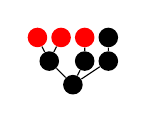
\begin{tikzpicture}[scale=.2]
\node[circle, scale=0.75, fill] (tid0) at (3,0){};
\node[circle, scale=0.75, fill] (tid1) at (1.5,1.5){};
\node[circle, scale=0.75, fill, red] (tid4) at (0.75,3){};
\node[circle, scale=0.75, fill, red] (tid5) at (2.25,3){};
\draw[](tid1) -- (tid4);
\draw[](tid1) -- (tid5);
\node[circle, scale=0.75, fill] (tid2) at (3.75,1.5){};
\node[circle, scale=0.75, fill, red] (tid6) at (3.75,3){};
\draw[](tid2) -- (tid6);
\node[circle, scale=0.75, fill] (tid3) at (5.25,1.5){};
\node[circle, scale=0.75, fill] (tid7) at (5.25,3){};
\draw[](tid3) -- (tid7);
\draw[](tid0) -- (tid1);
\draw[](tid0) -- (tid2);
\draw[](tid0) -- (tid3);

\end{tikzpicture}
\nodepart{two}
\footnotesize{4.54321}
\nodepart{three}
\footnotesize{$67\:33$}
};
\node[draw=black, rectangle split, rectangle split parts=3] (sn0x8fdea28W-12) at (-12, -48) {
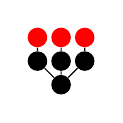
\begin{tikzpicture}[scale=.2]
\node[circle, scale=0.75, fill] (tid0) at (2.25,0){};
\node[circle, scale=0.75, fill] (tid1) at (0.75,1.5){};
\node[circle, scale=0.75, fill, red] (tid4) at (0.75,3){};
\draw[](tid1) -- (tid4);
\node[circle, scale=0.75, fill] (tid2) at (2.25,1.5){};
\node[circle, scale=0.75, fill, red] (tid5) at (2.25,3){};
\draw[](tid2) -- (tid5);
\node[circle, scale=0.75, fill] (tid3) at (3.75,1.5){};
\node[circle, scale=0.75, fill, red] (tid6) at (3.75,3){};
\draw[](tid3) -- (tid6);
\draw[](tid0) -- (tid1);
\draw[](tid0) -- (tid2);
\draw[](tid0) -- (tid3);

\end{tikzpicture}
\nodepart{two}
\footnotesize{4.21296}
\nodepart{three}
\footnotesize{$1$}
};
\node[draw=black, rectangle split, rectangle split parts=3] (sn0x8fd8170W-7) at (-7.25, -60) {
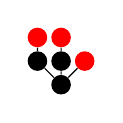
\begin{tikzpicture}[scale=.2]
\node[circle, scale=0.75, fill] (tid0) at (2.25,0){};
\node[circle, scale=0.75, fill] (tid1) at (0.75,1.5){};
\node[circle, scale=0.75, fill, red] (tid4) at (0.75,3){};
\draw[](tid1) -- (tid4);
\node[circle, scale=0.75, fill] (tid2) at (2.25,1.5){};
\node[circle, scale=0.75, fill, red] (tid5) at (2.25,3){};
\draw[](tid2) -- (tid5);
\node[circle, scale=0.75, fill, red] (tid3) at (3.75,1.5){};
\draw[](tid0) -- (tid1);
\draw[](tid0) -- (tid2);
\draw[](tid0) -- (tid3);

\end{tikzpicture}
\nodepart{two}
\footnotesize{3.87963}
\nodepart{three}
\footnotesize{$33\:67$}
};
\node[draw=black, rectangle split, rectangle split parts=3] (sn0x8fd6e28W-9) at (-9, -72) {
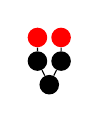
\begin{tikzpicture}[scale=.2]
\node[circle, scale=0.75, fill] (tid0) at (1.5,0){};
\node[circle, scale=0.75, fill] (tid1) at (0.75,1.5){};
\node[circle, scale=0.75, fill, red] (tid3) at (0.75,3){};
\draw[](tid1) -- (tid3);
\node[circle, scale=0.75, fill] (tid2) at (2.25,1.5){};
\node[circle, scale=0.75, fill, red] (tid4) at (2.25,3){};
\draw[](tid2) -- (tid4);
\draw[](tid0) -- (tid1);
\draw[](tid0) -- (tid2);

\end{tikzpicture}
\nodepart{two}
\footnotesize{3.75}
\nodepart{three}
\footnotesize{$1$}
};
\node[draw=black, rectangle split, rectangle split parts=3] (sn0x8fd3e80W-8) at (-8.25, -84) {
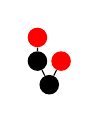
\begin{tikzpicture}[scale=.2]
\node[circle, scale=0.75, fill] (tid0) at (1.5,0){};
\node[circle, scale=0.75, fill] (tid1) at (0.75,1.5){};
\node[circle, scale=0.75, fill, red] (tid3) at (0.75,3){};
\draw[](tid1) -- (tid3);
\node[circle, scale=0.75, fill, red] (tid2) at (2.25,1.5){};
\draw[](tid0) -- (tid1);
\draw[](tid0) -- (tid2);

\end{tikzpicture}
\nodepart{two}
\footnotesize{3.25}
\nodepart{three}
\footnotesize{$50\:50$}
};
\node[draw=black, rectangle split, rectangle split parts=3] (sn0x8fd75a8W-4) at (-4.25, -96) {
\begin{tikzpicture}[scale=.2]
\node[circle, scale=0.75, fill] (tid0) at (0.75,0){};
\node[circle, scale=0.75, fill] (tid1) at (0.75,1.5){};
\node[circle, scale=0.75, fill, red] (tid2) at (0.75,3){};
\draw[](tid1) -- (tid2);
\draw[](tid0) -- (tid1);

\end{tikzpicture}
\nodepart{two}
\footnotesize{3}
\nodepart{three}
\footnotesize{$1$}
};
\node[draw=black, rectangle split, rectangle split parts=3] (sn0x8fd30e8W-1) at (-1.75, -108) {
\begin{tikzpicture}[scale=.2]
\node[circle, scale=0.75, fill] (tid0) at (0.75,0){};
\node[circle, scale=0.75, fill, red] (tid1) at (0.75,1.5){};
\draw[](tid0) -- (tid1);

\end{tikzpicture}
\nodepart{two}
\footnotesize{2}
\nodepart{three}
\footnotesize{$1$}
};
\draw (sn0x8fd75a8W-4.south) -- (sn0x8fd30e8W-1.north);
\node[draw=black, rectangle split, rectangle split parts=3] (sn0x8fd3158W0) at (-0.75, -96) {
\begin{tikzpicture}[scale=.2]
\node[circle, scale=0.75, fill] (tid0) at (1.5,0){};
\node[circle, scale=0.75, fill, red] (tid1) at (0.75,1.5){};
\node[circle, scale=0.75, fill, red] (tid2) at (2.25,1.5){};
\draw[](tid0) -- (tid1);
\draw[](tid0) -- (tid2);

\end{tikzpicture}
\nodepart{two}
\footnotesize{2.5}
\nodepart{three}
\footnotesize{$1$}
};
\draw (sn0x8fd3158W0.south) -- (sn0x8fd30e8W-1.north);
\draw (sn0x8fd3e80W-8.south) -- (sn0x8fd75a8W-4.north);
\draw (sn0x8fd3e80W-8.south) -- (sn0x8fd3158W0.north);
\draw (sn0x8fd6e28W-9.south) -- (sn0x8fd3e80W-8.north);
\node[draw=black, rectangle split, rectangle split parts=3] (sn0x8fd4d48W-4) at (-4, -72) {
\begin{tikzpicture}[scale=.2]
\node[circle, scale=0.75, fill] (tid0) at (2.25,0){};
\node[circle, scale=0.75, fill] (tid1) at (0.75,1.5){};
\node[circle, scale=0.75, fill, red] (tid4) at (0.75,3){};
\draw[](tid1) -- (tid4);
\node[circle, scale=0.75, fill, red] (tid2) at (2.25,1.5){};
\node[circle, scale=0.75, fill, red] (tid3) at (3.75,1.5){};
\draw[](tid0) -- (tid1);
\draw[](tid0) -- (tid2);
\draw[](tid0) -- (tid3);

\end{tikzpicture}
\nodepart{two}
\footnotesize{3.44444}
\nodepart{three}
\footnotesize{$67\:33$}
};
\node[draw=black, rectangle split, rectangle split parts=3] (sn0x8fd58e8W-3) at (-3.25, -84) {
\begin{tikzpicture}[scale=.2]
\node[circle, scale=0.75, fill] (tid0) at (2.25,0){};
\node[circle, scale=0.75, fill, red] (tid1) at (0.75,1.5){};
\node[circle, scale=0.75, fill, red] (tid2) at (2.25,1.5){};
\node[circle, scale=0.75, fill, red] (tid3) at (3.75,1.5){};
\draw[](tid0) -- (tid1);
\draw[](tid0) -- (tid2);
\draw[](tid0) -- (tid3);

\end{tikzpicture}
\nodepart{two}
\footnotesize{2.83333}
\nodepart{three}
\footnotesize{$1$}
};
\draw (sn0x8fd58e8W-3.south) -- (sn0x8fd3158W0.north);
\draw (sn0x8fd4d48W-4.south) -- (sn0x8fd3e80W-8.north);
\draw (sn0x8fd4d48W-4.south) -- (sn0x8fd58e8W-3.north);
\draw (sn0x8fd8170W-7.south) -- (sn0x8fd6e28W-9.north);
\draw (sn0x8fd8170W-7.south) -- (sn0x8fd4d48W-4.north);
\draw (sn0x8fdea28W-12.south) -- (sn0x8fd8170W-7.north);
\node[draw=black, rectangle split, rectangle split parts=3] (sn0x8fd6cf8W-5) at (-5.5, -48) {
\begin{tikzpicture}[scale=.2]
\node[circle, scale=0.75, fill] (tid0) at (3,0){};
\node[circle, scale=0.75, fill] (tid1) at (1.5,1.5){};
\node[circle, scale=0.75, fill, red] (tid4) at (0.75,3){};
\node[circle, scale=0.75, fill, red] (tid5) at (2.25,3){};
\draw[](tid1) -- (tid4);
\draw[](tid1) -- (tid5);
\node[circle, scale=0.75, fill] (tid2) at (3.75,1.5){};
\node[circle, scale=0.75, fill, red] (tid6) at (3.75,3){};
\draw[](tid2) -- (tid6);
\node[circle, scale=0.75, fill] (tid3) at (5.25,1.5){};
\draw[](tid0) -- (tid1);
\draw[](tid0) -- (tid2);
\draw[](tid0) -- (tid3);

\end{tikzpicture}
\nodepart{two}
\footnotesize{4.2037}
\nodepart{three}
\footnotesize{$67\:33$}
};
\node[draw=black, rectangle split, rectangle split parts=3] (sn0x8fd6610W0) at (-0.75, -60) {
\begin{tikzpicture}[scale=.2]
\node[circle, scale=0.75, fill] (tid0) at (3,0){};
\node[circle, scale=0.75, fill] (tid1) at (1.5,1.5){};
\node[circle, scale=0.75, fill, red] (tid4) at (0.75,3){};
\node[circle, scale=0.75, fill, red] (tid5) at (2.25,3){};
\draw[](tid1) -- (tid4);
\draw[](tid1) -- (tid5);
\node[circle, scale=0.75, fill, red] (tid2) at (3.75,1.5){};
\node[circle, scale=0.75, fill] (tid3) at (5.25,1.5){};
\draw[](tid0) -- (tid1);
\draw[](tid0) -- (tid2);
\draw[](tid0) -- (tid3);

\end{tikzpicture}
\nodepart{two}
\footnotesize{3.85185}
\nodepart{three}
\footnotesize{$33\:67$}
};
\node[draw=black, rectangle split, rectangle split parts=3] (sn0x8fd7358W2) at (2.5, -72) {
\begin{tikzpicture}[scale=.2]
\node[circle, scale=0.75, fill] (tid0) at (2.25,0){};
\node[circle, scale=0.75, fill] (tid1) at (1.5,1.5){};
\node[circle, scale=0.75, fill, red] (tid3) at (0.75,3){};
\node[circle, scale=0.75, fill, red] (tid4) at (2.25,3){};
\draw[](tid1) -- (tid3);
\draw[](tid1) -- (tid4);
\node[circle, scale=0.75, fill, red] (tid2) at (3.75,1.5){};
\draw[](tid0) -- (tid1);
\draw[](tid0) -- (tid2);

\end{tikzpicture}
\nodepart{two}
\footnotesize{3.66667}
\nodepart{three}
\footnotesize{$33\:67$}
};
\node[draw=black, rectangle split, rectangle split parts=3] (sn0x8fd8a08W3) at (3.25, -84) {
\begin{tikzpicture}[scale=.2]
\node[circle, scale=0.75, fill] (tid0) at (1.5,0){};
\node[circle, scale=0.75, fill] (tid1) at (1.5,1.5){};
\node[circle, scale=0.75, fill, red] (tid2) at (0.75,3){};
\node[circle, scale=0.75, fill, red] (tid3) at (2.25,3){};
\draw[](tid1) -- (tid2);
\draw[](tid1) -- (tid3);
\draw[](tid0) -- (tid1);

\end{tikzpicture}
\nodepart{two}
\footnotesize{3.5}
\nodepart{three}
\footnotesize{$1$}
};
\draw (sn0x8fd8a08W3.south) -- (sn0x8fd75a8W-4.north);
\draw (sn0x8fd7358W2.south) -- (sn0x8fd8a08W3.north);
\draw (sn0x8fd7358W2.south) -- (sn0x8fd3e80W-8.north);
\draw (sn0x8fd6610W0.south) -- (sn0x8fd7358W2.north);
\draw (sn0x8fd6610W0.south) -- (sn0x8fd4d48W-4.north);
\draw (sn0x8fd6cf8W-5.south) -- (sn0x8fd8170W-7.north);
\draw (sn0x8fd6cf8W-5.south) -- (sn0x8fd6610W0.north);
\draw (sn0x8fd4e10W-22.south) -- (sn0x8fdea28W-12.north);
\draw (sn0x8fd4e10W-22.south) -- (sn0x8fd6cf8W-5.north);
\node[draw=black, rectangle split, rectangle split parts=3] (sn0x8fd3d30W-14) at (-14.25, -36) {
\begin{tikzpicture}[scale=.2]
\node[circle, scale=0.75, fill] (tid0) at (3,0){};
\node[circle, scale=0.75, fill] (tid1) at (1.5,1.5){};
\node[circle, scale=0.75, fill, red] (tid4) at (0.75,3){};
\node[circle, scale=0.75, fill] (tid5) at (2.25,3){};
\draw[](tid1) -- (tid4);
\draw[](tid1) -- (tid5);
\node[circle, scale=0.75, fill] (tid2) at (3.75,1.5){};
\node[circle, scale=0.75, fill, red] (tid6) at (3.75,3){};
\draw[](tid2) -- (tid6);
\node[circle, scale=0.75, fill] (tid3) at (5.25,1.5){};
\node[circle, scale=0.75, fill, red] (tid7) at (5.25,3){};
\draw[](tid3) -- (tid7);
\draw[](tid0) -- (tid1);
\draw[](tid0) -- (tid2);
\draw[](tid0) -- (tid3);

\end{tikzpicture}
\nodepart{two}
\footnotesize{4.54012}
\nodepart{three}
\footnotesize{$33\:67$}
};
\draw (sn0x8fd3d30W-14.south) -- (sn0x8fdea28W-12.north);
\draw (sn0x8fd3d30W-14.south) -- (sn0x8fd6cf8W-5.north);
\draw (sn0x8fdf1c8W-19.south) -- (sn0x8fd4e10W-22.north);
\draw (sn0x8fdf1c8W-19.south) -- (sn0x8fd3d30W-14.north);
\node[draw=black, rectangle split, rectangle split parts=3] (sn0x8fd3e00W-9) at (-9.5, -24) {
\begin{tikzpicture}[scale=.2]
\node[circle, scale=0.75, fill] (tid0) at (3.75,0){};
\node[circle, scale=0.75, fill] (tid1) at (1.5,1.5){};
\node[circle, scale=0.75, fill, red] (tid4) at (0.75,3){};
\node[circle, scale=0.75, fill] (tid5) at (2.25,3){};
\draw[](tid1) -- (tid4);
\draw[](tid1) -- (tid5);
\node[circle, scale=0.75, fill] (tid2) at (4.5,1.5){};
\node[circle, scale=0.75, fill, red] (tid6) at (3.75,3){};
\node[circle, scale=0.75, fill] (tid7) at (5.25,3){};
\draw[](tid2) -- (tid6);
\draw[](tid2) -- (tid7);
\node[circle, scale=0.75, fill] (tid3) at (6.75,1.5){};
\node[circle, scale=0.75, fill, red] (tid8) at (6.75,3){};
\draw[](tid3) -- (tid8);
\draw[](tid0) -- (tid1);
\draw[](tid0) -- (tid2);
\draw[](tid0) -- (tid3);

\end{tikzpicture}
\nodepart{two}
\footnotesize{4.87346}
\nodepart{three}
\footnotesize{$33\:33\:33$}
};
\node[draw=black, rectangle split, rectangle split parts=3] (sn0x8fde270W-6) at (-6.25, -36) {
\begin{tikzpicture}[scale=.2]
\node[circle, scale=0.75, fill] (tid0) at (3.75,0){};
\node[circle, scale=0.75, fill] (tid1) at (1.5,1.5){};
\node[circle, scale=0.75, fill, red] (tid4) at (0.75,3){};
\node[circle, scale=0.75, fill, red] (tid5) at (2.25,3){};
\draw[](tid1) -- (tid4);
\draw[](tid1) -- (tid5);
\node[circle, scale=0.75, fill] (tid2) at (4.5,1.5){};
\node[circle, scale=0.75, fill, red] (tid6) at (3.75,3){};
\node[circle, scale=0.75, fill] (tid7) at (5.25,3){};
\draw[](tid2) -- (tid6);
\draw[](tid2) -- (tid7);
\node[circle, scale=0.75, fill] (tid3) at (6.75,1.5){};
\draw[](tid0) -- (tid1);
\draw[](tid0) -- (tid2);
\draw[](tid0) -- (tid3);

\end{tikzpicture}
\nodepart{two}
\footnotesize{4.53704}
\nodepart{three}
\footnotesize{$1$}
};
\draw (sn0x8fde270W-6.south) -- (sn0x8fd6cf8W-5.north);
\draw (sn0x8fd3e00W-9.south) -- (sn0x8fd3d30W-14.north);
\draw (sn0x8fd3e00W-9.south) -- (sn0x8fd4e10W-22.north);
\draw (sn0x8fd3e00W-9.south) -- (sn0x8fde270W-6.north);
\node[draw=black, rectangle split, rectangle split parts=3] (sn0x8fdfd90W0) at (0, -24) {
\begin{tikzpicture}[scale=.2]
\node[circle, scale=0.75, fill] (tid0) at (3.75,0){};
\node[circle, scale=0.75, fill] (tid1) at (2.25,1.5){};
\node[circle, scale=0.75, fill, red] (tid4) at (0.75,3){};
\node[circle, scale=0.75, fill, red] (tid5) at (2.25,3){};
\node[circle, scale=0.75, fill, red] (tid6) at (3.75,3){};
\draw[](tid1) -- (tid4);
\draw[](tid1) -- (tid5);
\draw[](tid1) -- (tid6);
\node[circle, scale=0.75, fill] (tid2) at (5.25,1.5){};
\node[circle, scale=0.75, fill] (tid7) at (5.25,3){};
\draw[](tid2) -- (tid7);
\node[circle, scale=0.75, fill] (tid3) at (6.75,1.5){};
\node[circle, scale=0.75, fill] (tid8) at (6.75,3){};
\draw[](tid3) -- (tid8);
\draw[](tid0) -- (tid1);
\draw[](tid0) -- (tid2);
\draw[](tid0) -- (tid3);

\end{tikzpicture}
\nodepart{two}
\footnotesize{4.87654}
\nodepart{three}
\footnotesize{$1$}
};
\draw (sn0x8fdfd90W0.south) -- (sn0x8fd4e10W-22.north);
\node[draw=black, rectangle split, rectangle split parts=3] (sn0x8fe00d0W9) at (9.5, -24) {
\begin{tikzpicture}[scale=.2]
\node[circle, scale=0.75, fill] (tid0) at (3.75,0){};
\node[circle, scale=0.75, fill] (tid1) at (2.25,1.5){};
\node[circle, scale=0.75, fill, red] (tid4) at (0.75,3){};
\node[circle, scale=0.75, fill, red] (tid5) at (2.25,3){};
\node[circle, scale=0.75, fill] (tid6) at (3.75,3){};
\draw[](tid1) -- (tid4);
\draw[](tid1) -- (tid5);
\draw[](tid1) -- (tid6);
\node[circle, scale=0.75, fill] (tid2) at (5.25,1.5){};
\node[circle, scale=0.75, fill, red] (tid7) at (5.25,3){};
\draw[](tid2) -- (tid7);
\node[circle, scale=0.75, fill] (tid3) at (6.75,1.5){};
\node[circle, scale=0.75, fill] (tid8) at (6.75,3){};
\draw[](tid3) -- (tid8);
\draw[](tid0) -- (tid1);
\draw[](tid0) -- (tid2);
\draw[](tid0) -- (tid3);

\end{tikzpicture}
\nodepart{two}
\footnotesize{4.87243}
\nodepart{three}
\footnotesize{$33\:33\:17\:17$}
};
\node[draw=black, rectangle split, rectangle split parts=3] (sn0x8fdefe0W3) at (3.25, -36) {
\begin{tikzpicture}[scale=.2]
\node[circle, scale=0.75, fill] (tid0) at (3.75,0){};
\node[circle, scale=0.75, fill] (tid1) at (2.25,1.5){};
\node[circle, scale=0.75, fill, red] (tid4) at (0.75,3){};
\node[circle, scale=0.75, fill, red] (tid5) at (2.25,3){};
\node[circle, scale=0.75, fill, red] (tid6) at (3.75,3){};
\draw[](tid1) -- (tid4);
\draw[](tid1) -- (tid5);
\draw[](tid1) -- (tid6);
\node[circle, scale=0.75, fill] (tid2) at (5.25,1.5){};
\node[circle, scale=0.75, fill] (tid7) at (5.25,3){};
\draw[](tid2) -- (tid7);
\node[circle, scale=0.75, fill] (tid3) at (6.75,1.5){};
\draw[](tid0) -- (tid1);
\draw[](tid0) -- (tid2);
\draw[](tid0) -- (tid3);

\end{tikzpicture}
\nodepart{two}
\footnotesize{4.53704}
\nodepart{three}
\footnotesize{$1$}
};
\draw (sn0x8fdefe0W3.south) -- (sn0x8fd6cf8W-5.north);
\node[draw=black, rectangle split, rectangle split parts=3] (sn0x8fde610W12) at (12.75, -36) {
\begin{tikzpicture}[scale=.2]
\node[circle, scale=0.75, fill] (tid0) at (3.75,0){};
\node[circle, scale=0.75, fill] (tid1) at (2.25,1.5){};
\node[circle, scale=0.75, fill, red] (tid4) at (0.75,3){};
\node[circle, scale=0.75, fill, red] (tid5) at (2.25,3){};
\node[circle, scale=0.75, fill] (tid6) at (3.75,3){};
\draw[](tid1) -- (tid4);
\draw[](tid1) -- (tid5);
\draw[](tid1) -- (tid6);
\node[circle, scale=0.75, fill] (tid2) at (5.25,1.5){};
\node[circle, scale=0.75, fill, red] (tid7) at (5.25,3){};
\draw[](tid2) -- (tid7);
\node[circle, scale=0.75, fill] (tid3) at (6.75,1.5){};
\draw[](tid0) -- (tid1);
\draw[](tid0) -- (tid2);
\draw[](tid0) -- (tid3);

\end{tikzpicture}
\nodepart{two}
\footnotesize{4.53086}
\nodepart{three}
\footnotesize{$67\:33$}
};
\node[draw=black, rectangle split, rectangle split parts=3] (sn0x8fdf3d0W2) at (2.5, -48) {
\begin{tikzpicture}[scale=.2]
\node[circle, scale=0.75, fill] (tid0) at (3.75,0){};
\node[circle, scale=0.75, fill] (tid1) at (2.25,1.5){};
\node[circle, scale=0.75, fill, red] (tid4) at (0.75,3){};
\node[circle, scale=0.75, fill, red] (tid5) at (2.25,3){};
\node[circle, scale=0.75, fill, red] (tid6) at (3.75,3){};
\draw[](tid1) -- (tid4);
\draw[](tid1) -- (tid5);
\draw[](tid1) -- (tid6);
\node[circle, scale=0.75, fill] (tid2) at (5.25,1.5){};
\node[circle, scale=0.75, fill] (tid3) at (6.75,1.5){};
\draw[](tid0) -- (tid1);
\draw[](tid0) -- (tid2);
\draw[](tid0) -- (tid3);

\end{tikzpicture}
\nodepart{two}
\footnotesize{4.18519}
\nodepart{three}
\footnotesize{$1$}
};
\draw (sn0x8fdf3d0W2.south) -- (sn0x8fd6610W0.north);
\draw (sn0x8fde610W12.south) -- (sn0x8fd6cf8W-5.north);
\draw (sn0x8fde610W12.south) -- (sn0x8fdf3d0W2.north);
\draw (sn0x8fe00d0W9.south) -- (sn0x8fd4e10W-22.north);
\draw (sn0x8fe00d0W9.south) -- (sn0x8fd3d30W-14.north);
\draw (sn0x8fe00d0W9.south) -- (sn0x8fdefe0W3.north);
\draw (sn0x8fe00d0W9.south) -- (sn0x8fde610W12.north);
\draw (sn0x8fd4440W-5.south) -- (sn0x8fdf1c8W-19.north);
\draw (sn0x8fd4440W-5.south) -- (sn0x8fd3e00W-9.north);
\draw (sn0x8fd4440W-5.south) -- (sn0x8fdfd90W0.north);
\draw (sn0x8fd4440W-5.south) -- (sn0x8fe00d0W9.north);
\end{tikzpicture}

%%% Local Variables:
%%% TeX-master: "thesis/thesis.tex"
%%% End: 

\begin{tikzpicture}[scale=.2, anchor=south west]
\node[draw=black, rectangle split, rectangle split parts=3] (sn0x8fd44a0W-5) at (-5.5, -12) {
\begin{tikzpicture}[scale=.2]
\node[circle, scale=0.75, fill] (tid0) at (4.5,0){};
\node[circle, scale=0.75, fill] (tid1) at (2.25,1.5){};
\node[circle, scale=0.75, fill, red] (tid4) at (0.75,3){};
\node[circle, scale=0.75, fill] (tid5) at (2.25,3){};
\node[circle, scale=0.75, fill] (tid6) at (3.75,3){};
\draw[](tid1) -- (tid4);
\draw[](tid1) -- (tid5);
\draw[](tid1) -- (tid6);
\node[circle, scale=0.75, fill] (tid2) at (6,1.5){};
\node[circle, scale=0.75, fill, red] (tid7) at (5.25,3){};
\node[circle, scale=0.75, fill] (tid8) at (6.75,3){};
\draw[](tid2) -- (tid7);
\draw[](tid2) -- (tid8);
\node[circle, scale=0.75, fill] (tid3) at (8.25,1.5){};
\node[circle, scale=0.75, fill, red] (tid9) at (8.25,3){};
\draw[](tid3) -- (tid9);
\draw[](tid0) -- (tid1);
\draw[](tid0) -- (tid2);
\draw[](tid0) -- (tid3);

\end{tikzpicture}
\nodepart{two}
\footnotesize{5.20405}
\nodepart{three}
\footnotesize{$22\:11\:22\:11\:22\:11$}
};
\node[draw=black, rectangle split, rectangle split parts=3] (sn0x8fd3e00W-30) at (-30, -24) {
\begin{tikzpicture}[scale=.2]
\node[circle, scale=0.75, fill] (tid0) at (3.75,0){};
\node[circle, scale=0.75, fill] (tid1) at (1.5,1.5){};
\node[circle, scale=0.75, fill, red] (tid4) at (0.75,3){};
\node[circle, scale=0.75, fill] (tid5) at (2.25,3){};
\draw[](tid1) -- (tid4);
\draw[](tid1) -- (tid5);
\node[circle, scale=0.75, fill] (tid2) at (4.5,1.5){};
\node[circle, scale=0.75, fill, red] (tid6) at (3.75,3){};
\node[circle, scale=0.75, fill] (tid7) at (5.25,3){};
\draw[](tid2) -- (tid6);
\draw[](tid2) -- (tid7);
\node[circle, scale=0.75, fill] (tid3) at (6.75,1.5){};
\node[circle, scale=0.75, fill, red] (tid8) at (6.75,3){};
\draw[](tid3) -- (tid8);
\draw[](tid0) -- (tid1);
\draw[](tid0) -- (tid2);
\draw[](tid0) -- (tid3);

\end{tikzpicture}
\nodepart{two}
\footnotesize{4.87346}
\nodepart{three}
\footnotesize{$33\:33\:33$}
};
\node[draw=black, rectangle split, rectangle split parts=3] (sn0x8fd3d30W-22) at (-22.25, -36) {
\begin{tikzpicture}[scale=.2]
\node[circle, scale=0.75, fill] (tid0) at (3,0){};
\node[circle, scale=0.75, fill] (tid1) at (1.5,1.5){};
\node[circle, scale=0.75, fill, red] (tid4) at (0.75,3){};
\node[circle, scale=0.75, fill] (tid5) at (2.25,3){};
\draw[](tid1) -- (tid4);
\draw[](tid1) -- (tid5);
\node[circle, scale=0.75, fill] (tid2) at (3.75,1.5){};
\node[circle, scale=0.75, fill, red] (tid6) at (3.75,3){};
\draw[](tid2) -- (tid6);
\node[circle, scale=0.75, fill] (tid3) at (5.25,1.5){};
\node[circle, scale=0.75, fill, red] (tid7) at (5.25,3){};
\draw[](tid3) -- (tid7);
\draw[](tid0) -- (tid1);
\draw[](tid0) -- (tid2);
\draw[](tid0) -- (tid3);

\end{tikzpicture}
\nodepart{two}
\footnotesize{4.54012}
\nodepart{three}
\footnotesize{$33\:67$}
};
\node[draw=black, rectangle split, rectangle split parts=3] (sn0x8fdea28W-12) at (-12, -48) {
\begin{tikzpicture}[scale=.2]
\node[circle, scale=0.75, fill] (tid0) at (2.25,0){};
\node[circle, scale=0.75, fill] (tid1) at (0.75,1.5){};
\node[circle, scale=0.75, fill, red] (tid4) at (0.75,3){};
\draw[](tid1) -- (tid4);
\node[circle, scale=0.75, fill] (tid2) at (2.25,1.5){};
\node[circle, scale=0.75, fill, red] (tid5) at (2.25,3){};
\draw[](tid2) -- (tid5);
\node[circle, scale=0.75, fill] (tid3) at (3.75,1.5){};
\node[circle, scale=0.75, fill, red] (tid6) at (3.75,3){};
\draw[](tid3) -- (tid6);
\draw[](tid0) -- (tid1);
\draw[](tid0) -- (tid2);
\draw[](tid0) -- (tid3);

\end{tikzpicture}
\nodepart{two}
\footnotesize{4.21296}
\nodepart{three}
\footnotesize{$1$}
};
\node[draw=black, rectangle split, rectangle split parts=3] (sn0x8fd8170W-7) at (-7.25, -60) {
\begin{tikzpicture}[scale=.2]
\node[circle, scale=0.75, fill] (tid0) at (2.25,0){};
\node[circle, scale=0.75, fill] (tid1) at (0.75,1.5){};
\node[circle, scale=0.75, fill, red] (tid4) at (0.75,3){};
\draw[](tid1) -- (tid4);
\node[circle, scale=0.75, fill] (tid2) at (2.25,1.5){};
\node[circle, scale=0.75, fill, red] (tid5) at (2.25,3){};
\draw[](tid2) -- (tid5);
\node[circle, scale=0.75, fill, red] (tid3) at (3.75,1.5){};
\draw[](tid0) -- (tid1);
\draw[](tid0) -- (tid2);
\draw[](tid0) -- (tid3);

\end{tikzpicture}
\nodepart{two}
\footnotesize{3.87963}
\nodepart{three}
\footnotesize{$33\:67$}
};
\node[draw=black, rectangle split, rectangle split parts=3] (sn0x8fd6e28W-9) at (-9, -72) {
\begin{tikzpicture}[scale=.2]
\node[circle, scale=0.75, fill] (tid0) at (1.5,0){};
\node[circle, scale=0.75, fill] (tid1) at (0.75,1.5){};
\node[circle, scale=0.75, fill, red] (tid3) at (0.75,3){};
\draw[](tid1) -- (tid3);
\node[circle, scale=0.75, fill] (tid2) at (2.25,1.5){};
\node[circle, scale=0.75, fill, red] (tid4) at (2.25,3){};
\draw[](tid2) -- (tid4);
\draw[](tid0) -- (tid1);
\draw[](tid0) -- (tid2);

\end{tikzpicture}
\nodepart{two}
\footnotesize{3.75}
\nodepart{three}
\footnotesize{$1$}
};
\node[draw=black, rectangle split, rectangle split parts=3] (sn0x8fd3e80W-8) at (-8.25, -84) {
\begin{tikzpicture}[scale=.2]
\node[circle, scale=0.75, fill] (tid0) at (1.5,0){};
\node[circle, scale=0.75, fill] (tid1) at (0.75,1.5){};
\node[circle, scale=0.75, fill, red] (tid3) at (0.75,3){};
\draw[](tid1) -- (tid3);
\node[circle, scale=0.75, fill, red] (tid2) at (2.25,1.5){};
\draw[](tid0) -- (tid1);
\draw[](tid0) -- (tid2);

\end{tikzpicture}
\nodepart{two}
\footnotesize{3.25}
\nodepart{three}
\footnotesize{$50\:50$}
};
\node[draw=black, rectangle split, rectangle split parts=3] (sn0x8fd75a8W-4) at (-4.25, -96) {
\begin{tikzpicture}[scale=.2]
\node[circle, scale=0.75, fill] (tid0) at (0.75,0){};
\node[circle, scale=0.75, fill] (tid1) at (0.75,1.5){};
\node[circle, scale=0.75, fill, red] (tid2) at (0.75,3){};
\draw[](tid1) -- (tid2);
\draw[](tid0) -- (tid1);

\end{tikzpicture}
\nodepart{two}
\footnotesize{3}
\nodepart{three}
\footnotesize{$1$}
};
\node[draw=black, rectangle split, rectangle split parts=3] (sn0x8fd30e8W-1) at (-1.75, -108) {
\begin{tikzpicture}[scale=.2]
\node[circle, scale=0.75, fill] (tid0) at (0.75,0){};
\node[circle, scale=0.75, fill, red] (tid1) at (0.75,1.5){};
\draw[](tid0) -- (tid1);

\end{tikzpicture}
\nodepart{two}
\footnotesize{2}
\nodepart{three}
\footnotesize{$1$}
};
\draw (sn0x8fd75a8W-4.south) -- (sn0x8fd30e8W-1.north);
\node[draw=black, rectangle split, rectangle split parts=3] (sn0x8fd3158W0) at (-0.75, -96) {
\begin{tikzpicture}[scale=.2]
\node[circle, scale=0.75, fill] (tid0) at (1.5,0){};
\node[circle, scale=0.75, fill, red] (tid1) at (0.75,1.5){};
\node[circle, scale=0.75, fill, red] (tid2) at (2.25,1.5){};
\draw[](tid0) -- (tid1);
\draw[](tid0) -- (tid2);

\end{tikzpicture}
\nodepart{two}
\footnotesize{2.5}
\nodepart{three}
\footnotesize{$1$}
};
\draw (sn0x8fd3158W0.south) -- (sn0x8fd30e8W-1.north);
\draw (sn0x8fd3e80W-8.south) -- (sn0x8fd75a8W-4.north);
\draw (sn0x8fd3e80W-8.south) -- (sn0x8fd3158W0.north);
\draw (sn0x8fd6e28W-9.south) -- (sn0x8fd3e80W-8.north);
\node[draw=black, rectangle split, rectangle split parts=3] (sn0x8fd4d48W-4) at (-4, -72) {
\begin{tikzpicture}[scale=.2]
\node[circle, scale=0.75, fill] (tid0) at (2.25,0){};
\node[circle, scale=0.75, fill] (tid1) at (0.75,1.5){};
\node[circle, scale=0.75, fill, red] (tid4) at (0.75,3){};
\draw[](tid1) -- (tid4);
\node[circle, scale=0.75, fill, red] (tid2) at (2.25,1.5){};
\node[circle, scale=0.75, fill, red] (tid3) at (3.75,1.5){};
\draw[](tid0) -- (tid1);
\draw[](tid0) -- (tid2);
\draw[](tid0) -- (tid3);

\end{tikzpicture}
\nodepart{two}
\footnotesize{3.44444}
\nodepart{three}
\footnotesize{$67\:33$}
};
\node[draw=black, rectangle split, rectangle split parts=3] (sn0x8fd58e8W-3) at (-3.25, -84) {
\begin{tikzpicture}[scale=.2]
\node[circle, scale=0.75, fill] (tid0) at (2.25,0){};
\node[circle, scale=0.75, fill, red] (tid1) at (0.75,1.5){};
\node[circle, scale=0.75, fill, red] (tid2) at (2.25,1.5){};
\node[circle, scale=0.75, fill, red] (tid3) at (3.75,1.5){};
\draw[](tid0) -- (tid1);
\draw[](tid0) -- (tid2);
\draw[](tid0) -- (tid3);

\end{tikzpicture}
\nodepart{two}
\footnotesize{2.83333}
\nodepart{three}
\footnotesize{$1$}
};
\draw (sn0x8fd58e8W-3.south) -- (sn0x8fd3158W0.north);
\draw (sn0x8fd4d48W-4.south) -- (sn0x8fd3e80W-8.north);
\draw (sn0x8fd4d48W-4.south) -- (sn0x8fd58e8W-3.north);
\draw (sn0x8fd8170W-7.south) -- (sn0x8fd6e28W-9.north);
\draw (sn0x8fd8170W-7.south) -- (sn0x8fd4d48W-4.north);
\draw (sn0x8fdea28W-12.south) -- (sn0x8fd8170W-7.north);
\node[draw=black, rectangle split, rectangle split parts=3] (sn0x8fd6cf8W-5) at (-5.5, -48) {
\begin{tikzpicture}[scale=.2]
\node[circle, scale=0.75, fill] (tid0) at (3,0){};
\node[circle, scale=0.75, fill] (tid1) at (1.5,1.5){};
\node[circle, scale=0.75, fill, red] (tid4) at (0.75,3){};
\node[circle, scale=0.75, fill, red] (tid5) at (2.25,3){};
\draw[](tid1) -- (tid4);
\draw[](tid1) -- (tid5);
\node[circle, scale=0.75, fill] (tid2) at (3.75,1.5){};
\node[circle, scale=0.75, fill, red] (tid6) at (3.75,3){};
\draw[](tid2) -- (tid6);
\node[circle, scale=0.75, fill] (tid3) at (5.25,1.5){};
\draw[](tid0) -- (tid1);
\draw[](tid0) -- (tid2);
\draw[](tid0) -- (tid3);

\end{tikzpicture}
\nodepart{two}
\footnotesize{4.2037}
\nodepart{three}
\footnotesize{$67\:33$}
};
\node[draw=black, rectangle split, rectangle split parts=3] (sn0x8fd6610W0) at (-0.75, -60) {
\begin{tikzpicture}[scale=.2]
\node[circle, scale=0.75, fill] (tid0) at (3,0){};
\node[circle, scale=0.75, fill] (tid1) at (1.5,1.5){};
\node[circle, scale=0.75, fill, red] (tid4) at (0.75,3){};
\node[circle, scale=0.75, fill, red] (tid5) at (2.25,3){};
\draw[](tid1) -- (tid4);
\draw[](tid1) -- (tid5);
\node[circle, scale=0.75, fill, red] (tid2) at (3.75,1.5){};
\node[circle, scale=0.75, fill] (tid3) at (5.25,1.5){};
\draw[](tid0) -- (tid1);
\draw[](tid0) -- (tid2);
\draw[](tid0) -- (tid3);

\end{tikzpicture}
\nodepart{two}
\footnotesize{3.85185}
\nodepart{three}
\footnotesize{$33\:67$}
};
\node[draw=black, rectangle split, rectangle split parts=3] (sn0x8fd7358W2) at (2.5, -72) {
\begin{tikzpicture}[scale=.2]
\node[circle, scale=0.75, fill] (tid0) at (2.25,0){};
\node[circle, scale=0.75, fill] (tid1) at (1.5,1.5){};
\node[circle, scale=0.75, fill, red] (tid3) at (0.75,3){};
\node[circle, scale=0.75, fill, red] (tid4) at (2.25,3){};
\draw[](tid1) -- (tid3);
\draw[](tid1) -- (tid4);
\node[circle, scale=0.75, fill, red] (tid2) at (3.75,1.5){};
\draw[](tid0) -- (tid1);
\draw[](tid0) -- (tid2);

\end{tikzpicture}
\nodepart{two}
\footnotesize{3.66667}
\nodepart{three}
\footnotesize{$33\:67$}
};
\node[draw=black, rectangle split, rectangle split parts=3] (sn0x8fd8a08W3) at (3.25, -84) {
\begin{tikzpicture}[scale=.2]
\node[circle, scale=0.75, fill] (tid0) at (1.5,0){};
\node[circle, scale=0.75, fill] (tid1) at (1.5,1.5){};
\node[circle, scale=0.75, fill, red] (tid2) at (0.75,3){};
\node[circle, scale=0.75, fill, red] (tid3) at (2.25,3){};
\draw[](tid1) -- (tid2);
\draw[](tid1) -- (tid3);
\draw[](tid0) -- (tid1);

\end{tikzpicture}
\nodepart{two}
\footnotesize{3.5}
\nodepart{three}
\footnotesize{$1$}
};
\draw (sn0x8fd8a08W3.south) -- (sn0x8fd75a8W-4.north);
\draw (sn0x8fd7358W2.south) -- (sn0x8fd8a08W3.north);
\draw (sn0x8fd7358W2.south) -- (sn0x8fd3e80W-8.north);
\draw (sn0x8fd6610W0.south) -- (sn0x8fd7358W2.north);
\draw (sn0x8fd6610W0.south) -- (sn0x8fd4d48W-4.north);
\draw (sn0x8fd6cf8W-5.south) -- (sn0x8fd8170W-7.north);
\draw (sn0x8fd6cf8W-5.south) -- (sn0x8fd6610W0.north);
\draw (sn0x8fd3d30W-22.south) -- (sn0x8fdea28W-12.north);
\draw (sn0x8fd3d30W-22.south) -- (sn0x8fd6cf8W-5.north);
\node[draw=black, rectangle split, rectangle split parts=3] (sn0x8fd4e10W-14) at (-14.25, -36) {
\begin{tikzpicture}[scale=.2]
\node[circle, scale=0.75, fill] (tid0) at (3,0){};
\node[circle, scale=0.75, fill] (tid1) at (1.5,1.5){};
\node[circle, scale=0.75, fill, red] (tid4) at (0.75,3){};
\node[circle, scale=0.75, fill, red] (tid5) at (2.25,3){};
\draw[](tid1) -- (tid4);
\draw[](tid1) -- (tid5);
\node[circle, scale=0.75, fill] (tid2) at (3.75,1.5){};
\node[circle, scale=0.75, fill, red] (tid6) at (3.75,3){};
\draw[](tid2) -- (tid6);
\node[circle, scale=0.75, fill] (tid3) at (5.25,1.5){};
\node[circle, scale=0.75, fill] (tid7) at (5.25,3){};
\draw[](tid3) -- (tid7);
\draw[](tid0) -- (tid1);
\draw[](tid0) -- (tid2);
\draw[](tid0) -- (tid3);

\end{tikzpicture}
\nodepart{two}
\footnotesize{4.54321}
\nodepart{three}
\footnotesize{$67\:33$}
};
\draw (sn0x8fd4e10W-14.south) -- (sn0x8fdea28W-12.north);
\draw (sn0x8fd4e10W-14.south) -- (sn0x8fd6cf8W-5.north);
\node[draw=black, rectangle split, rectangle split parts=3] (sn0x8fde270W-6) at (-6.25, -36) {
\begin{tikzpicture}[scale=.2]
\node[circle, scale=0.75, fill] (tid0) at (3.75,0){};
\node[circle, scale=0.75, fill] (tid1) at (1.5,1.5){};
\node[circle, scale=0.75, fill, red] (tid4) at (0.75,3){};
\node[circle, scale=0.75, fill, red] (tid5) at (2.25,3){};
\draw[](tid1) -- (tid4);
\draw[](tid1) -- (tid5);
\node[circle, scale=0.75, fill] (tid2) at (4.5,1.5){};
\node[circle, scale=0.75, fill, red] (tid6) at (3.75,3){};
\node[circle, scale=0.75, fill] (tid7) at (5.25,3){};
\draw[](tid2) -- (tid6);
\draw[](tid2) -- (tid7);
\node[circle, scale=0.75, fill] (tid3) at (6.75,1.5){};
\draw[](tid0) -- (tid1);
\draw[](tid0) -- (tid2);
\draw[](tid0) -- (tid3);

\end{tikzpicture}
\nodepart{two}
\footnotesize{4.53704}
\nodepart{three}
\footnotesize{$1$}
};
\draw (sn0x8fde270W-6.south) -- (sn0x8fd6cf8W-5.north);
\draw (sn0x8fd3e00W-30.south) -- (sn0x8fd3d30W-22.north);
\draw (sn0x8fd3e00W-30.south) -- (sn0x8fd4e10W-14.north);
\draw (sn0x8fd3e00W-30.south) -- (sn0x8fde270W-6.north);
\node[draw=black, rectangle split, rectangle split parts=3] (sn0x8fd3f88W-20) at (-20.5, -24) {
\begin{tikzpicture}[scale=.2]
\node[circle, scale=0.75, fill] (tid0) at (3.75,0){};
\node[circle, scale=0.75, fill] (tid1) at (1.5,1.5){};
\node[circle, scale=0.75, fill, red] (tid4) at (0.75,3){};
\node[circle, scale=0.75, fill, red] (tid5) at (2.25,3){};
\draw[](tid1) -- (tid4);
\draw[](tid1) -- (tid5);
\node[circle, scale=0.75, fill] (tid2) at (4.5,1.5){};
\node[circle, scale=0.75, fill] (tid6) at (3.75,3){};
\node[circle, scale=0.75, fill] (tid7) at (5.25,3){};
\draw[](tid2) -- (tid6);
\draw[](tid2) -- (tid7);
\node[circle, scale=0.75, fill] (tid3) at (6.75,1.5){};
\node[circle, scale=0.75, fill, red] (tid8) at (6.75,3){};
\draw[](tid3) -- (tid8);
\draw[](tid0) -- (tid1);
\draw[](tid0) -- (tid2);
\draw[](tid0) -- (tid3);

\end{tikzpicture}
\nodepart{two}
\footnotesize{4.87243}
\nodepart{three}
\footnotesize{$67\:33$}
};
\draw (sn0x8fd3f88W-20.south) -- (sn0x8fd3d30W-22.north);
\draw (sn0x8fd3f88W-20.south) -- (sn0x8fde270W-6.north);
\node[draw=black, rectangle split, rectangle split parts=3] (sn0x8fe00d0W-11) at (-11, -24) {
\begin{tikzpicture}[scale=.2]
\node[circle, scale=0.75, fill] (tid0) at (3.75,0){};
\node[circle, scale=0.75, fill] (tid1) at (2.25,1.5){};
\node[circle, scale=0.75, fill, red] (tid4) at (0.75,3){};
\node[circle, scale=0.75, fill, red] (tid5) at (2.25,3){};
\node[circle, scale=0.75, fill] (tid6) at (3.75,3){};
\draw[](tid1) -- (tid4);
\draw[](tid1) -- (tid5);
\draw[](tid1) -- (tid6);
\node[circle, scale=0.75, fill] (tid2) at (5.25,1.5){};
\node[circle, scale=0.75, fill, red] (tid7) at (5.25,3){};
\draw[](tid2) -- (tid7);
\node[circle, scale=0.75, fill] (tid3) at (6.75,1.5){};
\node[circle, scale=0.75, fill] (tid8) at (6.75,3){};
\draw[](tid3) -- (tid8);
\draw[](tid0) -- (tid1);
\draw[](tid0) -- (tid2);
\draw[](tid0) -- (tid3);

\end{tikzpicture}
\nodepart{two}
\footnotesize{4.87243}
\nodepart{three}
\footnotesize{$33\:33\:17\:17$}
};
\node[draw=black, rectangle split, rectangle split parts=3] (sn0x8fdefe0W3) at (3.25, -36) {
\begin{tikzpicture}[scale=.2]
\node[circle, scale=0.75, fill] (tid0) at (3.75,0){};
\node[circle, scale=0.75, fill] (tid1) at (2.25,1.5){};
\node[circle, scale=0.75, fill, red] (tid4) at (0.75,3){};
\node[circle, scale=0.75, fill, red] (tid5) at (2.25,3){};
\node[circle, scale=0.75, fill, red] (tid6) at (3.75,3){};
\draw[](tid1) -- (tid4);
\draw[](tid1) -- (tid5);
\draw[](tid1) -- (tid6);
\node[circle, scale=0.75, fill] (tid2) at (5.25,1.5){};
\node[circle, scale=0.75, fill] (tid7) at (5.25,3){};
\draw[](tid2) -- (tid7);
\node[circle, scale=0.75, fill] (tid3) at (6.75,1.5){};
\draw[](tid0) -- (tid1);
\draw[](tid0) -- (tid2);
\draw[](tid0) -- (tid3);

\end{tikzpicture}
\nodepart{two}
\footnotesize{4.53704}
\nodepart{three}
\footnotesize{$1$}
};
\draw (sn0x8fdefe0W3.south) -- (sn0x8fd6cf8W-5.north);
\node[draw=black, rectangle split, rectangle split parts=3] (sn0x8fde610W12) at (12.75, -36) {
\begin{tikzpicture}[scale=.2]
\node[circle, scale=0.75, fill] (tid0) at (3.75,0){};
\node[circle, scale=0.75, fill] (tid1) at (2.25,1.5){};
\node[circle, scale=0.75, fill, red] (tid4) at (0.75,3){};
\node[circle, scale=0.75, fill, red] (tid5) at (2.25,3){};
\node[circle, scale=0.75, fill] (tid6) at (3.75,3){};
\draw[](tid1) -- (tid4);
\draw[](tid1) -- (tid5);
\draw[](tid1) -- (tid6);
\node[circle, scale=0.75, fill] (tid2) at (5.25,1.5){};
\node[circle, scale=0.75, fill, red] (tid7) at (5.25,3){};
\draw[](tid2) -- (tid7);
\node[circle, scale=0.75, fill] (tid3) at (6.75,1.5){};
\draw[](tid0) -- (tid1);
\draw[](tid0) -- (tid2);
\draw[](tid0) -- (tid3);

\end{tikzpicture}
\nodepart{two}
\footnotesize{4.53086}
\nodepart{three}
\footnotesize{$67\:33$}
};
\node[draw=black, rectangle split, rectangle split parts=3] (sn0x8fdf3d0W2) at (2.5, -48) {
\begin{tikzpicture}[scale=.2]
\node[circle, scale=0.75, fill] (tid0) at (3.75,0){};
\node[circle, scale=0.75, fill] (tid1) at (2.25,1.5){};
\node[circle, scale=0.75, fill, red] (tid4) at (0.75,3){};
\node[circle, scale=0.75, fill, red] (tid5) at (2.25,3){};
\node[circle, scale=0.75, fill, red] (tid6) at (3.75,3){};
\draw[](tid1) -- (tid4);
\draw[](tid1) -- (tid5);
\draw[](tid1) -- (tid6);
\node[circle, scale=0.75, fill] (tid2) at (5.25,1.5){};
\node[circle, scale=0.75, fill] (tid3) at (6.75,1.5){};
\draw[](tid0) -- (tid1);
\draw[](tid0) -- (tid2);
\draw[](tid0) -- (tid3);

\end{tikzpicture}
\nodepart{two}
\footnotesize{4.18519}
\nodepart{three}
\footnotesize{$1$}
};
\draw (sn0x8fdf3d0W2.south) -- (sn0x8fd6610W0.north);
\draw (sn0x8fde610W12.south) -- (sn0x8fd6cf8W-5.north);
\draw (sn0x8fde610W12.south) -- (sn0x8fdf3d0W2.north);
\draw (sn0x8fe00d0W-11.south) -- (sn0x8fd4e10W-14.north);
\draw (sn0x8fe00d0W-11.south) -- (sn0x8fd3d30W-22.north);
\draw (sn0x8fe00d0W-11.south) -- (sn0x8fdefe0W3.north);
\draw (sn0x8fe00d0W-11.south) -- (sn0x8fde610W12.north);
\node[draw=black, rectangle split, rectangle split parts=3] (sn0x8fe0458W-1) at (-1.5, -24) {
\begin{tikzpicture}[scale=.2]
\node[circle, scale=0.75, fill] (tid0) at (3.75,0){};
\node[circle, scale=0.75, fill] (tid1) at (2.25,1.5){};
\node[circle, scale=0.75, fill, red] (tid4) at (0.75,3){};
\node[circle, scale=0.75, fill] (tid5) at (2.25,3){};
\node[circle, scale=0.75, fill] (tid6) at (3.75,3){};
\draw[](tid1) -- (tid4);
\draw[](tid1) -- (tid5);
\draw[](tid1) -- (tid6);
\node[circle, scale=0.75, fill] (tid2) at (5.25,1.5){};
\node[circle, scale=0.75, fill, red] (tid7) at (5.25,3){};
\draw[](tid2) -- (tid7);
\node[circle, scale=0.75, fill] (tid3) at (6.75,1.5){};
\node[circle, scale=0.75, fill, red] (tid8) at (6.75,3){};
\draw[](tid3) -- (tid8);
\draw[](tid0) -- (tid1);
\draw[](tid0) -- (tid2);
\draw[](tid0) -- (tid3);

\end{tikzpicture}
\nodepart{two}
\footnotesize{4.86728}
\nodepart{three}
\footnotesize{$33\:67$}
};
\draw (sn0x8fe0458W-1.south) -- (sn0x8fd3d30W-22.north);
\draw (sn0x8fe0458W-1.south) -- (sn0x8fde610W12.north);
\node[draw=black, rectangle split, rectangle split parts=3] (sn0x8fd34c8W8) at (8, -24) {
\begin{tikzpicture}[scale=.2]
\node[circle, scale=0.75, fill] (tid0) at (4.5,0){};
\node[circle, scale=0.75, fill] (tid1) at (2.25,1.5){};
\node[circle, scale=0.75, fill, red] (tid4) at (0.75,3){};
\node[circle, scale=0.75, fill, red] (tid5) at (2.25,3){};
\node[circle, scale=0.75, fill] (tid6) at (3.75,3){};
\draw[](tid1) -- (tid4);
\draw[](tid1) -- (tid5);
\draw[](tid1) -- (tid6);
\node[circle, scale=0.75, fill] (tid2) at (6,1.5){};
\node[circle, scale=0.75, fill, red] (tid7) at (5.25,3){};
\node[circle, scale=0.75, fill] (tid8) at (6.75,3){};
\draw[](tid2) -- (tid7);
\draw[](tid2) -- (tid8);
\node[circle, scale=0.75, fill] (tid3) at (8.25,1.5){};
\draw[](tid0) -- (tid1);
\draw[](tid0) -- (tid2);
\draw[](tid0) -- (tid3);

\end{tikzpicture}
\nodepart{two}
\footnotesize{4.86934}
\nodepart{three}
\footnotesize{$67\:17\:17$}
};
\draw (sn0x8fd34c8W8.south) -- (sn0x8fde270W-6.north);
\draw (sn0x8fd34c8W8.south) -- (sn0x8fdefe0W3.north);
\draw (sn0x8fd34c8W8.south) -- (sn0x8fde610W12.north);
\node[draw=black, rectangle split, rectangle split parts=3] (sn0x8fe04c0W19) at (19, -24) {
\begin{tikzpicture}[scale=.2]
\node[circle, scale=0.75, fill] (tid0) at (4.5,0){};
\node[circle, scale=0.75, fill] (tid1) at (2.25,1.5){};
\node[circle, scale=0.75, fill, red] (tid4) at (0.75,3){};
\node[circle, scale=0.75, fill] (tid5) at (2.25,3){};
\node[circle, scale=0.75, fill] (tid6) at (3.75,3){};
\draw[](tid1) -- (tid4);
\draw[](tid1) -- (tid5);
\draw[](tid1) -- (tid6);
\node[circle, scale=0.75, fill] (tid2) at (6,1.5){};
\node[circle, scale=0.75, fill, red] (tid7) at (5.25,3){};
\node[circle, scale=0.75, fill, red] (tid8) at (6.75,3){};
\draw[](tid2) -- (tid7);
\draw[](tid2) -- (tid8);
\node[circle, scale=0.75, fill] (tid3) at (8.25,1.5){};
\draw[](tid0) -- (tid1);
\draw[](tid0) -- (tid2);
\draw[](tid0) -- (tid3);

\end{tikzpicture}
\nodepart{two}
\footnotesize{4.86626}
\nodepart{three}
\footnotesize{$33\:67$}
};
\draw (sn0x8fe04c0W19.south) -- (sn0x8fde270W-6.north);
\draw (sn0x8fe04c0W19.south) -- (sn0x8fde610W12.north);
\draw (sn0x8fd44a0W-5.south) -- (sn0x8fd3e00W-30.north);
\draw (sn0x8fd44a0W-5.south) -- (sn0x8fd3f88W-20.north);
\draw (sn0x8fd44a0W-5.south) -- (sn0x8fe00d0W-11.north);
\draw (sn0x8fd44a0W-5.south) -- (sn0x8fe0458W-1.north);
\draw (sn0x8fd44a0W-5.south) -- (sn0x8fd34c8W8.north);
\draw (sn0x8fd44a0W-5.south) -- (sn0x8fe04c0W19.north);
\end{tikzpicture}

%%% Local Variables:
%%% TeX-master: "thesis/thesis.tex"
%%% End: 

\begin{tikzpicture}[scale=.2, anchor=south west]
\node[draw=black, rectangle split, rectangle split parts=3] (sn0x8fd4500W-5) at (-5.5, -12) {
\begin{tikzpicture}[scale=.2]
\node[circle, scale=0.75, fill] (tid0) at (4.5,0){};
\node[circle, scale=0.75, fill] (tid1) at (2.25,1.5){};
\node[circle, scale=0.75, fill] (tid4) at (0.75,3){};
\node[circle, scale=0.75, fill] (tid5) at (2.25,3){};
\node[circle, scale=0.75, fill] (tid6) at (3.75,3){};
\draw[](tid1) -- (tid4);
\draw[](tid1) -- (tid5);
\draw[](tid1) -- (tid6);
\node[circle, scale=0.75, fill] (tid2) at (6,1.5){};
\node[circle, scale=0.75, fill, red] (tid7) at (5.25,3){};
\node[circle, scale=0.75, fill, red] (tid8) at (6.75,3){};
\draw[](tid2) -- (tid7);
\draw[](tid2) -- (tid8);
\node[circle, scale=0.75, fill] (tid3) at (8.25,1.5){};
\node[circle, scale=0.75, fill, red] (tid9) at (8.25,3){};
\draw[](tid3) -- (tid9);
\draw[](tid0) -- (tid1);
\draw[](tid0) -- (tid2);
\draw[](tid0) -- (tid3);

\end{tikzpicture}
\nodepart{two}
\footnotesize{5.20028}
\nodepart{three}
\footnotesize{$67\:33$}
};
\node[draw=black, rectangle split, rectangle split parts=3] (sn0x8fe0458W-10) at (-10.25, -24) {
\begin{tikzpicture}[scale=.2]
\node[circle, scale=0.75, fill] (tid0) at (3.75,0){};
\node[circle, scale=0.75, fill] (tid1) at (2.25,1.5){};
\node[circle, scale=0.75, fill, red] (tid4) at (0.75,3){};
\node[circle, scale=0.75, fill] (tid5) at (2.25,3){};
\node[circle, scale=0.75, fill] (tid6) at (3.75,3){};
\draw[](tid1) -- (tid4);
\draw[](tid1) -- (tid5);
\draw[](tid1) -- (tid6);
\node[circle, scale=0.75, fill] (tid2) at (5.25,1.5){};
\node[circle, scale=0.75, fill, red] (tid7) at (5.25,3){};
\draw[](tid2) -- (tid7);
\node[circle, scale=0.75, fill] (tid3) at (6.75,1.5){};
\node[circle, scale=0.75, fill, red] (tid8) at (6.75,3){};
\draw[](tid3) -- (tid8);
\draw[](tid0) -- (tid1);
\draw[](tid0) -- (tid2);
\draw[](tid0) -- (tid3);

\end{tikzpicture}
\nodepart{two}
\footnotesize{4.86728}
\nodepart{three}
\footnotesize{$33\:67$}
};
\node[draw=black, rectangle split, rectangle split parts=3] (sn0x8fd3d30W-13) at (-13.5, -36) {
\begin{tikzpicture}[scale=.2]
\node[circle, scale=0.75, fill] (tid0) at (3,0){};
\node[circle, scale=0.75, fill] (tid1) at (1.5,1.5){};
\node[circle, scale=0.75, fill, red] (tid4) at (0.75,3){};
\node[circle, scale=0.75, fill] (tid5) at (2.25,3){};
\draw[](tid1) -- (tid4);
\draw[](tid1) -- (tid5);
\node[circle, scale=0.75, fill] (tid2) at (3.75,1.5){};
\node[circle, scale=0.75, fill, red] (tid6) at (3.75,3){};
\draw[](tid2) -- (tid6);
\node[circle, scale=0.75, fill] (tid3) at (5.25,1.5){};
\node[circle, scale=0.75, fill, red] (tid7) at (5.25,3){};
\draw[](tid3) -- (tid7);
\draw[](tid0) -- (tid1);
\draw[](tid0) -- (tid2);
\draw[](tid0) -- (tid3);

\end{tikzpicture}
\nodepart{two}
\footnotesize{4.54012}
\nodepart{three}
\footnotesize{$33\:67$}
};
\node[draw=black, rectangle split, rectangle split parts=3] (sn0x8fdea28W-12) at (-12, -48) {
\begin{tikzpicture}[scale=.2]
\node[circle, scale=0.75, fill] (tid0) at (2.25,0){};
\node[circle, scale=0.75, fill] (tid1) at (0.75,1.5){};
\node[circle, scale=0.75, fill, red] (tid4) at (0.75,3){};
\draw[](tid1) -- (tid4);
\node[circle, scale=0.75, fill] (tid2) at (2.25,1.5){};
\node[circle, scale=0.75, fill, red] (tid5) at (2.25,3){};
\draw[](tid2) -- (tid5);
\node[circle, scale=0.75, fill] (tid3) at (3.75,1.5){};
\node[circle, scale=0.75, fill, red] (tid6) at (3.75,3){};
\draw[](tid3) -- (tid6);
\draw[](tid0) -- (tid1);
\draw[](tid0) -- (tid2);
\draw[](tid0) -- (tid3);

\end{tikzpicture}
\nodepart{two}
\footnotesize{4.21296}
\nodepart{three}
\footnotesize{$1$}
};
\node[draw=black, rectangle split, rectangle split parts=3] (sn0x8fd8170W-7) at (-7.25, -60) {
\begin{tikzpicture}[scale=.2]
\node[circle, scale=0.75, fill] (tid0) at (2.25,0){};
\node[circle, scale=0.75, fill] (tid1) at (0.75,1.5){};
\node[circle, scale=0.75, fill, red] (tid4) at (0.75,3){};
\draw[](tid1) -- (tid4);
\node[circle, scale=0.75, fill] (tid2) at (2.25,1.5){};
\node[circle, scale=0.75, fill, red] (tid5) at (2.25,3){};
\draw[](tid2) -- (tid5);
\node[circle, scale=0.75, fill, red] (tid3) at (3.75,1.5){};
\draw[](tid0) -- (tid1);
\draw[](tid0) -- (tid2);
\draw[](tid0) -- (tid3);

\end{tikzpicture}
\nodepart{two}
\footnotesize{3.87963}
\nodepart{three}
\footnotesize{$33\:67$}
};
\node[draw=black, rectangle split, rectangle split parts=3] (sn0x8fd6e28W-9) at (-9, -72) {
\begin{tikzpicture}[scale=.2]
\node[circle, scale=0.75, fill] (tid0) at (1.5,0){};
\node[circle, scale=0.75, fill] (tid1) at (0.75,1.5){};
\node[circle, scale=0.75, fill, red] (tid3) at (0.75,3){};
\draw[](tid1) -- (tid3);
\node[circle, scale=0.75, fill] (tid2) at (2.25,1.5){};
\node[circle, scale=0.75, fill, red] (tid4) at (2.25,3){};
\draw[](tid2) -- (tid4);
\draw[](tid0) -- (tid1);
\draw[](tid0) -- (tid2);

\end{tikzpicture}
\nodepart{two}
\footnotesize{3.75}
\nodepart{three}
\footnotesize{$1$}
};
\node[draw=black, rectangle split, rectangle split parts=3] (sn0x8fd3e80W-8) at (-8.25, -84) {
\begin{tikzpicture}[scale=.2]
\node[circle, scale=0.75, fill] (tid0) at (1.5,0){};
\node[circle, scale=0.75, fill] (tid1) at (0.75,1.5){};
\node[circle, scale=0.75, fill, red] (tid3) at (0.75,3){};
\draw[](tid1) -- (tid3);
\node[circle, scale=0.75, fill, red] (tid2) at (2.25,1.5){};
\draw[](tid0) -- (tid1);
\draw[](tid0) -- (tid2);

\end{tikzpicture}
\nodepart{two}
\footnotesize{3.25}
\nodepart{three}
\footnotesize{$50\:50$}
};
\node[draw=black, rectangle split, rectangle split parts=3] (sn0x8fd75a8W-4) at (-4.25, -96) {
\begin{tikzpicture}[scale=.2]
\node[circle, scale=0.75, fill] (tid0) at (0.75,0){};
\node[circle, scale=0.75, fill] (tid1) at (0.75,1.5){};
\node[circle, scale=0.75, fill, red] (tid2) at (0.75,3){};
\draw[](tid1) -- (tid2);
\draw[](tid0) -- (tid1);

\end{tikzpicture}
\nodepart{two}
\footnotesize{3}
\nodepart{three}
\footnotesize{$1$}
};
\node[draw=black, rectangle split, rectangle split parts=3] (sn0x8fd30e8W-1) at (-1.75, -108) {
\begin{tikzpicture}[scale=.2]
\node[circle, scale=0.75, fill] (tid0) at (0.75,0){};
\node[circle, scale=0.75, fill, red] (tid1) at (0.75,1.5){};
\draw[](tid0) -- (tid1);

\end{tikzpicture}
\nodepart{two}
\footnotesize{2}
\nodepart{three}
\footnotesize{$1$}
};
\draw (sn0x8fd75a8W-4.south) -- (sn0x8fd30e8W-1.north);
\node[draw=black, rectangle split, rectangle split parts=3] (sn0x8fd3158W0) at (-0.75, -96) {
\begin{tikzpicture}[scale=.2]
\node[circle, scale=0.75, fill] (tid0) at (1.5,0){};
\node[circle, scale=0.75, fill, red] (tid1) at (0.75,1.5){};
\node[circle, scale=0.75, fill, red] (tid2) at (2.25,1.5){};
\draw[](tid0) -- (tid1);
\draw[](tid0) -- (tid2);

\end{tikzpicture}
\nodepart{two}
\footnotesize{2.5}
\nodepart{three}
\footnotesize{$1$}
};
\draw (sn0x8fd3158W0.south) -- (sn0x8fd30e8W-1.north);
\draw (sn0x8fd3e80W-8.south) -- (sn0x8fd75a8W-4.north);
\draw (sn0x8fd3e80W-8.south) -- (sn0x8fd3158W0.north);
\draw (sn0x8fd6e28W-9.south) -- (sn0x8fd3e80W-8.north);
\node[draw=black, rectangle split, rectangle split parts=3] (sn0x8fd4d48W-4) at (-4, -72) {
\begin{tikzpicture}[scale=.2]
\node[circle, scale=0.75, fill] (tid0) at (2.25,0){};
\node[circle, scale=0.75, fill] (tid1) at (0.75,1.5){};
\node[circle, scale=0.75, fill, red] (tid4) at (0.75,3){};
\draw[](tid1) -- (tid4);
\node[circle, scale=0.75, fill, red] (tid2) at (2.25,1.5){};
\node[circle, scale=0.75, fill, red] (tid3) at (3.75,1.5){};
\draw[](tid0) -- (tid1);
\draw[](tid0) -- (tid2);
\draw[](tid0) -- (tid3);

\end{tikzpicture}
\nodepart{two}
\footnotesize{3.44444}
\nodepart{three}
\footnotesize{$67\:33$}
};
\node[draw=black, rectangle split, rectangle split parts=3] (sn0x8fd58e8W-3) at (-3.25, -84) {
\begin{tikzpicture}[scale=.2]
\node[circle, scale=0.75, fill] (tid0) at (2.25,0){};
\node[circle, scale=0.75, fill, red] (tid1) at (0.75,1.5){};
\node[circle, scale=0.75, fill, red] (tid2) at (2.25,1.5){};
\node[circle, scale=0.75, fill, red] (tid3) at (3.75,1.5){};
\draw[](tid0) -- (tid1);
\draw[](tid0) -- (tid2);
\draw[](tid0) -- (tid3);

\end{tikzpicture}
\nodepart{two}
\footnotesize{2.83333}
\nodepart{three}
\footnotesize{$1$}
};
\draw (sn0x8fd58e8W-3.south) -- (sn0x8fd3158W0.north);
\draw (sn0x8fd4d48W-4.south) -- (sn0x8fd3e80W-8.north);
\draw (sn0x8fd4d48W-4.south) -- (sn0x8fd58e8W-3.north);
\draw (sn0x8fd8170W-7.south) -- (sn0x8fd6e28W-9.north);
\draw (sn0x8fd8170W-7.south) -- (sn0x8fd4d48W-4.north);
\draw (sn0x8fdea28W-12.south) -- (sn0x8fd8170W-7.north);
\node[draw=black, rectangle split, rectangle split parts=3] (sn0x8fd6cf8W-5) at (-5.5, -48) {
\begin{tikzpicture}[scale=.2]
\node[circle, scale=0.75, fill] (tid0) at (3,0){};
\node[circle, scale=0.75, fill] (tid1) at (1.5,1.5){};
\node[circle, scale=0.75, fill, red] (tid4) at (0.75,3){};
\node[circle, scale=0.75, fill, red] (tid5) at (2.25,3){};
\draw[](tid1) -- (tid4);
\draw[](tid1) -- (tid5);
\node[circle, scale=0.75, fill] (tid2) at (3.75,1.5){};
\node[circle, scale=0.75, fill, red] (tid6) at (3.75,3){};
\draw[](tid2) -- (tid6);
\node[circle, scale=0.75, fill] (tid3) at (5.25,1.5){};
\draw[](tid0) -- (tid1);
\draw[](tid0) -- (tid2);
\draw[](tid0) -- (tid3);

\end{tikzpicture}
\nodepart{two}
\footnotesize{4.2037}
\nodepart{three}
\footnotesize{$67\:33$}
};
\node[draw=black, rectangle split, rectangle split parts=3] (sn0x8fd6610W0) at (-0.75, -60) {
\begin{tikzpicture}[scale=.2]
\node[circle, scale=0.75, fill] (tid0) at (3,0){};
\node[circle, scale=0.75, fill] (tid1) at (1.5,1.5){};
\node[circle, scale=0.75, fill, red] (tid4) at (0.75,3){};
\node[circle, scale=0.75, fill, red] (tid5) at (2.25,3){};
\draw[](tid1) -- (tid4);
\draw[](tid1) -- (tid5);
\node[circle, scale=0.75, fill, red] (tid2) at (3.75,1.5){};
\node[circle, scale=0.75, fill] (tid3) at (5.25,1.5){};
\draw[](tid0) -- (tid1);
\draw[](tid0) -- (tid2);
\draw[](tid0) -- (tid3);

\end{tikzpicture}
\nodepart{two}
\footnotesize{3.85185}
\nodepart{three}
\footnotesize{$33\:67$}
};
\node[draw=black, rectangle split, rectangle split parts=3] (sn0x8fd7358W2) at (2.5, -72) {
\begin{tikzpicture}[scale=.2]
\node[circle, scale=0.75, fill] (tid0) at (2.25,0){};
\node[circle, scale=0.75, fill] (tid1) at (1.5,1.5){};
\node[circle, scale=0.75, fill, red] (tid3) at (0.75,3){};
\node[circle, scale=0.75, fill, red] (tid4) at (2.25,3){};
\draw[](tid1) -- (tid3);
\draw[](tid1) -- (tid4);
\node[circle, scale=0.75, fill, red] (tid2) at (3.75,1.5){};
\draw[](tid0) -- (tid1);
\draw[](tid0) -- (tid2);

\end{tikzpicture}
\nodepart{two}
\footnotesize{3.66667}
\nodepart{three}
\footnotesize{$33\:67$}
};
\node[draw=black, rectangle split, rectangle split parts=3] (sn0x8fd8a08W3) at (3.25, -84) {
\begin{tikzpicture}[scale=.2]
\node[circle, scale=0.75, fill] (tid0) at (1.5,0){};
\node[circle, scale=0.75, fill] (tid1) at (1.5,1.5){};
\node[circle, scale=0.75, fill, red] (tid2) at (0.75,3){};
\node[circle, scale=0.75, fill, red] (tid3) at (2.25,3){};
\draw[](tid1) -- (tid2);
\draw[](tid1) -- (tid3);
\draw[](tid0) -- (tid1);

\end{tikzpicture}
\nodepart{two}
\footnotesize{3.5}
\nodepart{three}
\footnotesize{$1$}
};
\draw (sn0x8fd8a08W3.south) -- (sn0x8fd75a8W-4.north);
\draw (sn0x8fd7358W2.south) -- (sn0x8fd8a08W3.north);
\draw (sn0x8fd7358W2.south) -- (sn0x8fd3e80W-8.north);
\draw (sn0x8fd6610W0.south) -- (sn0x8fd7358W2.north);
\draw (sn0x8fd6610W0.south) -- (sn0x8fd4d48W-4.north);
\draw (sn0x8fd6cf8W-5.south) -- (sn0x8fd8170W-7.north);
\draw (sn0x8fd6cf8W-5.south) -- (sn0x8fd6610W0.north);
\draw (sn0x8fd3d30W-13.south) -- (sn0x8fdea28W-12.north);
\draw (sn0x8fd3d30W-13.south) -- (sn0x8fd6cf8W-5.north);
\node[draw=black, rectangle split, rectangle split parts=3] (sn0x8fde610W-5) at (-5.5, -36) {
\begin{tikzpicture}[scale=.2]
\node[circle, scale=0.75, fill] (tid0) at (3.75,0){};
\node[circle, scale=0.75, fill] (tid1) at (2.25,1.5){};
\node[circle, scale=0.75, fill, red] (tid4) at (0.75,3){};
\node[circle, scale=0.75, fill, red] (tid5) at (2.25,3){};
\node[circle, scale=0.75, fill] (tid6) at (3.75,3){};
\draw[](tid1) -- (tid4);
\draw[](tid1) -- (tid5);
\draw[](tid1) -- (tid6);
\node[circle, scale=0.75, fill] (tid2) at (5.25,1.5){};
\node[circle, scale=0.75, fill, red] (tid7) at (5.25,3){};
\draw[](tid2) -- (tid7);
\node[circle, scale=0.75, fill] (tid3) at (6.75,1.5){};
\draw[](tid0) -- (tid1);
\draw[](tid0) -- (tid2);
\draw[](tid0) -- (tid3);

\end{tikzpicture}
\nodepart{two}
\footnotesize{4.53086}
\nodepart{three}
\footnotesize{$67\:33$}
};
\node[draw=black, rectangle split, rectangle split parts=3] (sn0x8fdf3d0W2) at (2.5, -48) {
\begin{tikzpicture}[scale=.2]
\node[circle, scale=0.75, fill] (tid0) at (3.75,0){};
\node[circle, scale=0.75, fill] (tid1) at (2.25,1.5){};
\node[circle, scale=0.75, fill, red] (tid4) at (0.75,3){};
\node[circle, scale=0.75, fill, red] (tid5) at (2.25,3){};
\node[circle, scale=0.75, fill, red] (tid6) at (3.75,3){};
\draw[](tid1) -- (tid4);
\draw[](tid1) -- (tid5);
\draw[](tid1) -- (tid6);
\node[circle, scale=0.75, fill] (tid2) at (5.25,1.5){};
\node[circle, scale=0.75, fill] (tid3) at (6.75,1.5){};
\draw[](tid0) -- (tid1);
\draw[](tid0) -- (tid2);
\draw[](tid0) -- (tid3);

\end{tikzpicture}
\nodepart{two}
\footnotesize{4.18519}
\nodepart{three}
\footnotesize{$1$}
};
\draw (sn0x8fdf3d0W2.south) -- (sn0x8fd6610W0.north);
\draw (sn0x8fde610W-5.south) -- (sn0x8fd6cf8W-5.north);
\draw (sn0x8fde610W-5.south) -- (sn0x8fdf3d0W2.north);
\draw (sn0x8fe0458W-10.south) -- (sn0x8fd3d30W-13.north);
\draw (sn0x8fe0458W-10.south) -- (sn0x8fde610W-5.north);
\node[draw=black, rectangle split, rectangle split parts=3] (sn0x8fe04c0W0) at (-0.75, -24) {
\begin{tikzpicture}[scale=.2]
\node[circle, scale=0.75, fill] (tid0) at (4.5,0){};
\node[circle, scale=0.75, fill] (tid1) at (2.25,1.5){};
\node[circle, scale=0.75, fill, red] (tid4) at (0.75,3){};
\node[circle, scale=0.75, fill] (tid5) at (2.25,3){};
\node[circle, scale=0.75, fill] (tid6) at (3.75,3){};
\draw[](tid1) -- (tid4);
\draw[](tid1) -- (tid5);
\draw[](tid1) -- (tid6);
\node[circle, scale=0.75, fill] (tid2) at (6,1.5){};
\node[circle, scale=0.75, fill, red] (tid7) at (5.25,3){};
\node[circle, scale=0.75, fill, red] (tid8) at (6.75,3){};
\draw[](tid2) -- (tid7);
\draw[](tid2) -- (tid8);
\node[circle, scale=0.75, fill] (tid3) at (8.25,1.5){};
\draw[](tid0) -- (tid1);
\draw[](tid0) -- (tid2);
\draw[](tid0) -- (tid3);

\end{tikzpicture}
\nodepart{two}
\footnotesize{4.86626}
\nodepart{three}
\footnotesize{$33\:67$}
};
\node[draw=black, rectangle split, rectangle split parts=3] (sn0x8fde270W4) at (4, -36) {
\begin{tikzpicture}[scale=.2]
\node[circle, scale=0.75, fill] (tid0) at (3.75,0){};
\node[circle, scale=0.75, fill] (tid1) at (1.5,1.5){};
\node[circle, scale=0.75, fill, red] (tid4) at (0.75,3){};
\node[circle, scale=0.75, fill, red] (tid5) at (2.25,3){};
\draw[](tid1) -- (tid4);
\draw[](tid1) -- (tid5);
\node[circle, scale=0.75, fill] (tid2) at (4.5,1.5){};
\node[circle, scale=0.75, fill, red] (tid6) at (3.75,3){};
\node[circle, scale=0.75, fill] (tid7) at (5.25,3){};
\draw[](tid2) -- (tid6);
\draw[](tid2) -- (tid7);
\node[circle, scale=0.75, fill] (tid3) at (6.75,1.5){};
\draw[](tid0) -- (tid1);
\draw[](tid0) -- (tid2);
\draw[](tid0) -- (tid3);

\end{tikzpicture}
\nodepart{two}
\footnotesize{4.53704}
\nodepart{three}
\footnotesize{$1$}
};
\draw (sn0x8fde270W4.south) -- (sn0x8fd6cf8W-5.north);
\draw (sn0x8fe04c0W0.south) -- (sn0x8fde270W4.north);
\draw (sn0x8fe04c0W0.south) -- (sn0x8fde610W-5.north);
\draw (sn0x8fd4500W-5.south) -- (sn0x8fe0458W-10.north);
\draw (sn0x8fd4500W-5.south) -- (sn0x8fe04c0W0.north);
\end{tikzpicture}

%%% Local Variables:
%%% TeX-master: "thesis/thesis.tex"
%%% End: 

\begin{tikzpicture}[scale=.2, anchor=south west]
\node[draw=black, rectangle split, rectangle split parts=3] (sn0x8fd4560W-5) at (-5.5, -12) {
\begin{tikzpicture}[scale=.2]
\node[circle, scale=0.75, fill] (tid0) at (4.5,0){};
\node[circle, scale=0.75, fill] (tid1) at (2.25,1.5){};
\node[circle, scale=0.75, fill, red] (tid4) at (0.75,3){};
\node[circle, scale=0.75, fill] (tid5) at (2.25,3){};
\node[circle, scale=0.75, fill] (tid6) at (3.75,3){};
\draw[](tid1) -- (tid4);
\draw[](tid1) -- (tid5);
\draw[](tid1) -- (tid6);
\node[circle, scale=0.75, fill] (tid2) at (6,1.5){};
\node[circle, scale=0.75, fill, red] (tid7) at (5.25,3){};
\node[circle, scale=0.75, fill, red] (tid8) at (6.75,3){};
\draw[](tid2) -- (tid7);
\draw[](tid2) -- (tid8);
\node[circle, scale=0.75, fill] (tid3) at (8.25,1.5){};
\node[circle, scale=0.75, fill] (tid9) at (8.25,3){};
\draw[](tid3) -- (tid9);
\draw[](tid0) -- (tid1);
\draw[](tid0) -- (tid2);
\draw[](tid0) -- (tid3);

\end{tikzpicture}
\nodepart{two}
\footnotesize{5.20531}
\nodepart{three}
\footnotesize{$22\:11\:44\:22$}
};
\node[draw=black, rectangle split, rectangle split parts=3] (sn0x8fdf1c8W-19) at (-19, -24) {
\begin{tikzpicture}[scale=.2]
\node[circle, scale=0.75, fill] (tid0) at (3.75,0){};
\node[circle, scale=0.75, fill] (tid1) at (1.5,1.5){};
\node[circle, scale=0.75, fill, red] (tid4) at (0.75,3){};
\node[circle, scale=0.75, fill, red] (tid5) at (2.25,3){};
\draw[](tid1) -- (tid4);
\draw[](tid1) -- (tid5);
\node[circle, scale=0.75, fill] (tid2) at (4.5,1.5){};
\node[circle, scale=0.75, fill, red] (tid6) at (3.75,3){};
\node[circle, scale=0.75, fill] (tid7) at (5.25,3){};
\draw[](tid2) -- (tid6);
\draw[](tid2) -- (tid7);
\node[circle, scale=0.75, fill] (tid3) at (6.75,1.5){};
\node[circle, scale=0.75, fill] (tid8) at (6.75,3){};
\draw[](tid3) -- (tid8);
\draw[](tid0) -- (tid1);
\draw[](tid0) -- (tid2);
\draw[](tid0) -- (tid3);

\end{tikzpicture}
\nodepart{two}
\footnotesize{4.87551}
\nodepart{three}
\footnotesize{$67\:33$}
};
\node[draw=black, rectangle split, rectangle split parts=3] (sn0x8fd4e10W-22) at (-22.25, -36) {
\begin{tikzpicture}[scale=.2]
\node[circle, scale=0.75, fill] (tid0) at (3,0){};
\node[circle, scale=0.75, fill] (tid1) at (1.5,1.5){};
\node[circle, scale=0.75, fill, red] (tid4) at (0.75,3){};
\node[circle, scale=0.75, fill, red] (tid5) at (2.25,3){};
\draw[](tid1) -- (tid4);
\draw[](tid1) -- (tid5);
\node[circle, scale=0.75, fill] (tid2) at (3.75,1.5){};
\node[circle, scale=0.75, fill, red] (tid6) at (3.75,3){};
\draw[](tid2) -- (tid6);
\node[circle, scale=0.75, fill] (tid3) at (5.25,1.5){};
\node[circle, scale=0.75, fill] (tid7) at (5.25,3){};
\draw[](tid3) -- (tid7);
\draw[](tid0) -- (tid1);
\draw[](tid0) -- (tid2);
\draw[](tid0) -- (tid3);

\end{tikzpicture}
\nodepart{two}
\footnotesize{4.54321}
\nodepart{three}
\footnotesize{$67\:33$}
};
\node[draw=black, rectangle split, rectangle split parts=3] (sn0x8fdea28W-12) at (-12, -48) {
\begin{tikzpicture}[scale=.2]
\node[circle, scale=0.75, fill] (tid0) at (2.25,0){};
\node[circle, scale=0.75, fill] (tid1) at (0.75,1.5){};
\node[circle, scale=0.75, fill, red] (tid4) at (0.75,3){};
\draw[](tid1) -- (tid4);
\node[circle, scale=0.75, fill] (tid2) at (2.25,1.5){};
\node[circle, scale=0.75, fill, red] (tid5) at (2.25,3){};
\draw[](tid2) -- (tid5);
\node[circle, scale=0.75, fill] (tid3) at (3.75,1.5){};
\node[circle, scale=0.75, fill, red] (tid6) at (3.75,3){};
\draw[](tid3) -- (tid6);
\draw[](tid0) -- (tid1);
\draw[](tid0) -- (tid2);
\draw[](tid0) -- (tid3);

\end{tikzpicture}
\nodepart{two}
\footnotesize{4.21296}
\nodepart{three}
\footnotesize{$1$}
};
\node[draw=black, rectangle split, rectangle split parts=3] (sn0x8fd8170W-7) at (-7.25, -60) {
\begin{tikzpicture}[scale=.2]
\node[circle, scale=0.75, fill] (tid0) at (2.25,0){};
\node[circle, scale=0.75, fill] (tid1) at (0.75,1.5){};
\node[circle, scale=0.75, fill, red] (tid4) at (0.75,3){};
\draw[](tid1) -- (tid4);
\node[circle, scale=0.75, fill] (tid2) at (2.25,1.5){};
\node[circle, scale=0.75, fill, red] (tid5) at (2.25,3){};
\draw[](tid2) -- (tid5);
\node[circle, scale=0.75, fill, red] (tid3) at (3.75,1.5){};
\draw[](tid0) -- (tid1);
\draw[](tid0) -- (tid2);
\draw[](tid0) -- (tid3);

\end{tikzpicture}
\nodepart{two}
\footnotesize{3.87963}
\nodepart{three}
\footnotesize{$33\:67$}
};
\node[draw=black, rectangle split, rectangle split parts=3] (sn0x8fd6e28W-9) at (-9, -72) {
\begin{tikzpicture}[scale=.2]
\node[circle, scale=0.75, fill] (tid0) at (1.5,0){};
\node[circle, scale=0.75, fill] (tid1) at (0.75,1.5){};
\node[circle, scale=0.75, fill, red] (tid3) at (0.75,3){};
\draw[](tid1) -- (tid3);
\node[circle, scale=0.75, fill] (tid2) at (2.25,1.5){};
\node[circle, scale=0.75, fill, red] (tid4) at (2.25,3){};
\draw[](tid2) -- (tid4);
\draw[](tid0) -- (tid1);
\draw[](tid0) -- (tid2);

\end{tikzpicture}
\nodepart{two}
\footnotesize{3.75}
\nodepart{three}
\footnotesize{$1$}
};
\node[draw=black, rectangle split, rectangle split parts=3] (sn0x8fd3e80W-8) at (-8.25, -84) {
\begin{tikzpicture}[scale=.2]
\node[circle, scale=0.75, fill] (tid0) at (1.5,0){};
\node[circle, scale=0.75, fill] (tid1) at (0.75,1.5){};
\node[circle, scale=0.75, fill, red] (tid3) at (0.75,3){};
\draw[](tid1) -- (tid3);
\node[circle, scale=0.75, fill, red] (tid2) at (2.25,1.5){};
\draw[](tid0) -- (tid1);
\draw[](tid0) -- (tid2);

\end{tikzpicture}
\nodepart{two}
\footnotesize{3.25}
\nodepart{three}
\footnotesize{$50\:50$}
};
\node[draw=black, rectangle split, rectangle split parts=3] (sn0x8fd75a8W-4) at (-4.25, -96) {
\begin{tikzpicture}[scale=.2]
\node[circle, scale=0.75, fill] (tid0) at (0.75,0){};
\node[circle, scale=0.75, fill] (tid1) at (0.75,1.5){};
\node[circle, scale=0.75, fill, red] (tid2) at (0.75,3){};
\draw[](tid1) -- (tid2);
\draw[](tid0) -- (tid1);

\end{tikzpicture}
\nodepart{two}
\footnotesize{3}
\nodepart{three}
\footnotesize{$1$}
};
\node[draw=black, rectangle split, rectangle split parts=3] (sn0x8fd30e8W-1) at (-1.75, -108) {
\begin{tikzpicture}[scale=.2]
\node[circle, scale=0.75, fill] (tid0) at (0.75,0){};
\node[circle, scale=0.75, fill, red] (tid1) at (0.75,1.5){};
\draw[](tid0) -- (tid1);

\end{tikzpicture}
\nodepart{two}
\footnotesize{2}
\nodepart{three}
\footnotesize{$1$}
};
\draw (sn0x8fd75a8W-4.south) -- (sn0x8fd30e8W-1.north);
\node[draw=black, rectangle split, rectangle split parts=3] (sn0x8fd3158W0) at (-0.75, -96) {
\begin{tikzpicture}[scale=.2]
\node[circle, scale=0.75, fill] (tid0) at (1.5,0){};
\node[circle, scale=0.75, fill, red] (tid1) at (0.75,1.5){};
\node[circle, scale=0.75, fill, red] (tid2) at (2.25,1.5){};
\draw[](tid0) -- (tid1);
\draw[](tid0) -- (tid2);

\end{tikzpicture}
\nodepart{two}
\footnotesize{2.5}
\nodepart{three}
\footnotesize{$1$}
};
\draw (sn0x8fd3158W0.south) -- (sn0x8fd30e8W-1.north);
\draw (sn0x8fd3e80W-8.south) -- (sn0x8fd75a8W-4.north);
\draw (sn0x8fd3e80W-8.south) -- (sn0x8fd3158W0.north);
\draw (sn0x8fd6e28W-9.south) -- (sn0x8fd3e80W-8.north);
\node[draw=black, rectangle split, rectangle split parts=3] (sn0x8fd4d48W-4) at (-4, -72) {
\begin{tikzpicture}[scale=.2]
\node[circle, scale=0.75, fill] (tid0) at (2.25,0){};
\node[circle, scale=0.75, fill] (tid1) at (0.75,1.5){};
\node[circle, scale=0.75, fill, red] (tid4) at (0.75,3){};
\draw[](tid1) -- (tid4);
\node[circle, scale=0.75, fill, red] (tid2) at (2.25,1.5){};
\node[circle, scale=0.75, fill, red] (tid3) at (3.75,1.5){};
\draw[](tid0) -- (tid1);
\draw[](tid0) -- (tid2);
\draw[](tid0) -- (tid3);

\end{tikzpicture}
\nodepart{two}
\footnotesize{3.44444}
\nodepart{three}
\footnotesize{$67\:33$}
};
\node[draw=black, rectangle split, rectangle split parts=3] (sn0x8fd58e8W-3) at (-3.25, -84) {
\begin{tikzpicture}[scale=.2]
\node[circle, scale=0.75, fill] (tid0) at (2.25,0){};
\node[circle, scale=0.75, fill, red] (tid1) at (0.75,1.5){};
\node[circle, scale=0.75, fill, red] (tid2) at (2.25,1.5){};
\node[circle, scale=0.75, fill, red] (tid3) at (3.75,1.5){};
\draw[](tid0) -- (tid1);
\draw[](tid0) -- (tid2);
\draw[](tid0) -- (tid3);

\end{tikzpicture}
\nodepart{two}
\footnotesize{2.83333}
\nodepart{three}
\footnotesize{$1$}
};
\draw (sn0x8fd58e8W-3.south) -- (sn0x8fd3158W0.north);
\draw (sn0x8fd4d48W-4.south) -- (sn0x8fd3e80W-8.north);
\draw (sn0x8fd4d48W-4.south) -- (sn0x8fd58e8W-3.north);
\draw (sn0x8fd8170W-7.south) -- (sn0x8fd6e28W-9.north);
\draw (sn0x8fd8170W-7.south) -- (sn0x8fd4d48W-4.north);
\draw (sn0x8fdea28W-12.south) -- (sn0x8fd8170W-7.north);
\node[draw=black, rectangle split, rectangle split parts=3] (sn0x8fd6cf8W-5) at (-5.5, -48) {
\begin{tikzpicture}[scale=.2]
\node[circle, scale=0.75, fill] (tid0) at (3,0){};
\node[circle, scale=0.75, fill] (tid1) at (1.5,1.5){};
\node[circle, scale=0.75, fill, red] (tid4) at (0.75,3){};
\node[circle, scale=0.75, fill, red] (tid5) at (2.25,3){};
\draw[](tid1) -- (tid4);
\draw[](tid1) -- (tid5);
\node[circle, scale=0.75, fill] (tid2) at (3.75,1.5){};
\node[circle, scale=0.75, fill, red] (tid6) at (3.75,3){};
\draw[](tid2) -- (tid6);
\node[circle, scale=0.75, fill] (tid3) at (5.25,1.5){};
\draw[](tid0) -- (tid1);
\draw[](tid0) -- (tid2);
\draw[](tid0) -- (tid3);

\end{tikzpicture}
\nodepart{two}
\footnotesize{4.2037}
\nodepart{three}
\footnotesize{$67\:33$}
};
\node[draw=black, rectangle split, rectangle split parts=3] (sn0x8fd6610W0) at (-0.75, -60) {
\begin{tikzpicture}[scale=.2]
\node[circle, scale=0.75, fill] (tid0) at (3,0){};
\node[circle, scale=0.75, fill] (tid1) at (1.5,1.5){};
\node[circle, scale=0.75, fill, red] (tid4) at (0.75,3){};
\node[circle, scale=0.75, fill, red] (tid5) at (2.25,3){};
\draw[](tid1) -- (tid4);
\draw[](tid1) -- (tid5);
\node[circle, scale=0.75, fill, red] (tid2) at (3.75,1.5){};
\node[circle, scale=0.75, fill] (tid3) at (5.25,1.5){};
\draw[](tid0) -- (tid1);
\draw[](tid0) -- (tid2);
\draw[](tid0) -- (tid3);

\end{tikzpicture}
\nodepart{two}
\footnotesize{3.85185}
\nodepart{three}
\footnotesize{$33\:67$}
};
\node[draw=black, rectangle split, rectangle split parts=3] (sn0x8fd7358W2) at (2.5, -72) {
\begin{tikzpicture}[scale=.2]
\node[circle, scale=0.75, fill] (tid0) at (2.25,0){};
\node[circle, scale=0.75, fill] (tid1) at (1.5,1.5){};
\node[circle, scale=0.75, fill, red] (tid3) at (0.75,3){};
\node[circle, scale=0.75, fill, red] (tid4) at (2.25,3){};
\draw[](tid1) -- (tid3);
\draw[](tid1) -- (tid4);
\node[circle, scale=0.75, fill, red] (tid2) at (3.75,1.5){};
\draw[](tid0) -- (tid1);
\draw[](tid0) -- (tid2);

\end{tikzpicture}
\nodepart{two}
\footnotesize{3.66667}
\nodepart{three}
\footnotesize{$33\:67$}
};
\node[draw=black, rectangle split, rectangle split parts=3] (sn0x8fd8a08W3) at (3.25, -84) {
\begin{tikzpicture}[scale=.2]
\node[circle, scale=0.75, fill] (tid0) at (1.5,0){};
\node[circle, scale=0.75, fill] (tid1) at (1.5,1.5){};
\node[circle, scale=0.75, fill, red] (tid2) at (0.75,3){};
\node[circle, scale=0.75, fill, red] (tid3) at (2.25,3){};
\draw[](tid1) -- (tid2);
\draw[](tid1) -- (tid3);
\draw[](tid0) -- (tid1);

\end{tikzpicture}
\nodepart{two}
\footnotesize{3.5}
\nodepart{three}
\footnotesize{$1$}
};
\draw (sn0x8fd8a08W3.south) -- (sn0x8fd75a8W-4.north);
\draw (sn0x8fd7358W2.south) -- (sn0x8fd8a08W3.north);
\draw (sn0x8fd7358W2.south) -- (sn0x8fd3e80W-8.north);
\draw (sn0x8fd6610W0.south) -- (sn0x8fd7358W2.north);
\draw (sn0x8fd6610W0.south) -- (sn0x8fd4d48W-4.north);
\draw (sn0x8fd6cf8W-5.south) -- (sn0x8fd8170W-7.north);
\draw (sn0x8fd6cf8W-5.south) -- (sn0x8fd6610W0.north);
\draw (sn0x8fd4e10W-22.south) -- (sn0x8fdea28W-12.north);
\draw (sn0x8fd4e10W-22.south) -- (sn0x8fd6cf8W-5.north);
\node[draw=black, rectangle split, rectangle split parts=3] (sn0x8fd3d30W-14) at (-14.25, -36) {
\begin{tikzpicture}[scale=.2]
\node[circle, scale=0.75, fill] (tid0) at (3,0){};
\node[circle, scale=0.75, fill] (tid1) at (1.5,1.5){};
\node[circle, scale=0.75, fill, red] (tid4) at (0.75,3){};
\node[circle, scale=0.75, fill] (tid5) at (2.25,3){};
\draw[](tid1) -- (tid4);
\draw[](tid1) -- (tid5);
\node[circle, scale=0.75, fill] (tid2) at (3.75,1.5){};
\node[circle, scale=0.75, fill, red] (tid6) at (3.75,3){};
\draw[](tid2) -- (tid6);
\node[circle, scale=0.75, fill] (tid3) at (5.25,1.5){};
\node[circle, scale=0.75, fill, red] (tid7) at (5.25,3){};
\draw[](tid3) -- (tid7);
\draw[](tid0) -- (tid1);
\draw[](tid0) -- (tid2);
\draw[](tid0) -- (tid3);

\end{tikzpicture}
\nodepart{two}
\footnotesize{4.54012}
\nodepart{three}
\footnotesize{$33\:67$}
};
\draw (sn0x8fd3d30W-14.south) -- (sn0x8fdea28W-12.north);
\draw (sn0x8fd3d30W-14.south) -- (sn0x8fd6cf8W-5.north);
\draw (sn0x8fdf1c8W-19.south) -- (sn0x8fd4e10W-22.north);
\draw (sn0x8fdf1c8W-19.south) -- (sn0x8fd3d30W-14.north);
\node[draw=black, rectangle split, rectangle split parts=3] (sn0x8fd3f88W-9) at (-9.5, -24) {
\begin{tikzpicture}[scale=.2]
\node[circle, scale=0.75, fill] (tid0) at (3.75,0){};
\node[circle, scale=0.75, fill] (tid1) at (1.5,1.5){};
\node[circle, scale=0.75, fill, red] (tid4) at (0.75,3){};
\node[circle, scale=0.75, fill, red] (tid5) at (2.25,3){};
\draw[](tid1) -- (tid4);
\draw[](tid1) -- (tid5);
\node[circle, scale=0.75, fill] (tid2) at (4.5,1.5){};
\node[circle, scale=0.75, fill] (tid6) at (3.75,3){};
\node[circle, scale=0.75, fill] (tid7) at (5.25,3){};
\draw[](tid2) -- (tid6);
\draw[](tid2) -- (tid7);
\node[circle, scale=0.75, fill] (tid3) at (6.75,1.5){};
\node[circle, scale=0.75, fill, red] (tid8) at (6.75,3){};
\draw[](tid3) -- (tid8);
\draw[](tid0) -- (tid1);
\draw[](tid0) -- (tid2);
\draw[](tid0) -- (tid3);

\end{tikzpicture}
\nodepart{two}
\footnotesize{4.87243}
\nodepart{three}
\footnotesize{$67\:33$}
};
\node[draw=black, rectangle split, rectangle split parts=3] (sn0x8fde270W-6) at (-6.25, -36) {
\begin{tikzpicture}[scale=.2]
\node[circle, scale=0.75, fill] (tid0) at (3.75,0){};
\node[circle, scale=0.75, fill] (tid1) at (1.5,1.5){};
\node[circle, scale=0.75, fill, red] (tid4) at (0.75,3){};
\node[circle, scale=0.75, fill, red] (tid5) at (2.25,3){};
\draw[](tid1) -- (tid4);
\draw[](tid1) -- (tid5);
\node[circle, scale=0.75, fill] (tid2) at (4.5,1.5){};
\node[circle, scale=0.75, fill, red] (tid6) at (3.75,3){};
\node[circle, scale=0.75, fill] (tid7) at (5.25,3){};
\draw[](tid2) -- (tid6);
\draw[](tid2) -- (tid7);
\node[circle, scale=0.75, fill] (tid3) at (6.75,1.5){};
\draw[](tid0) -- (tid1);
\draw[](tid0) -- (tid2);
\draw[](tid0) -- (tid3);

\end{tikzpicture}
\nodepart{two}
\footnotesize{4.53704}
\nodepart{three}
\footnotesize{$1$}
};
\draw (sn0x8fde270W-6.south) -- (sn0x8fd6cf8W-5.north);
\draw (sn0x8fd3f88W-9.south) -- (sn0x8fd3d30W-14.north);
\draw (sn0x8fd3f88W-9.south) -- (sn0x8fde270W-6.north);
\node[draw=black, rectangle split, rectangle split parts=3] (sn0x8fe00d0W0) at (0, -24) {
\begin{tikzpicture}[scale=.2]
\node[circle, scale=0.75, fill] (tid0) at (3.75,0){};
\node[circle, scale=0.75, fill] (tid1) at (2.25,1.5){};
\node[circle, scale=0.75, fill, red] (tid4) at (0.75,3){};
\node[circle, scale=0.75, fill, red] (tid5) at (2.25,3){};
\node[circle, scale=0.75, fill] (tid6) at (3.75,3){};
\draw[](tid1) -- (tid4);
\draw[](tid1) -- (tid5);
\draw[](tid1) -- (tid6);
\node[circle, scale=0.75, fill] (tid2) at (5.25,1.5){};
\node[circle, scale=0.75, fill, red] (tid7) at (5.25,3){};
\draw[](tid2) -- (tid7);
\node[circle, scale=0.75, fill] (tid3) at (6.75,1.5){};
\node[circle, scale=0.75, fill] (tid8) at (6.75,3){};
\draw[](tid3) -- (tid8);
\draw[](tid0) -- (tid1);
\draw[](tid0) -- (tid2);
\draw[](tid0) -- (tid3);

\end{tikzpicture}
\nodepart{two}
\footnotesize{4.87243}
\nodepart{three}
\footnotesize{$33\:33\:17\:17$}
};
\node[draw=black, rectangle split, rectangle split parts=3] (sn0x8fdefe0W3) at (3.25, -36) {
\begin{tikzpicture}[scale=.2]
\node[circle, scale=0.75, fill] (tid0) at (3.75,0){};
\node[circle, scale=0.75, fill] (tid1) at (2.25,1.5){};
\node[circle, scale=0.75, fill, red] (tid4) at (0.75,3){};
\node[circle, scale=0.75, fill, red] (tid5) at (2.25,3){};
\node[circle, scale=0.75, fill, red] (tid6) at (3.75,3){};
\draw[](tid1) -- (tid4);
\draw[](tid1) -- (tid5);
\draw[](tid1) -- (tid6);
\node[circle, scale=0.75, fill] (tid2) at (5.25,1.5){};
\node[circle, scale=0.75, fill] (tid7) at (5.25,3){};
\draw[](tid2) -- (tid7);
\node[circle, scale=0.75, fill] (tid3) at (6.75,1.5){};
\draw[](tid0) -- (tid1);
\draw[](tid0) -- (tid2);
\draw[](tid0) -- (tid3);

\end{tikzpicture}
\nodepart{two}
\footnotesize{4.53704}
\nodepart{three}
\footnotesize{$1$}
};
\draw (sn0x8fdefe0W3.south) -- (sn0x8fd6cf8W-5.north);
\node[draw=black, rectangle split, rectangle split parts=3] (sn0x8fde610W12) at (12.75, -36) {
\begin{tikzpicture}[scale=.2]
\node[circle, scale=0.75, fill] (tid0) at (3.75,0){};
\node[circle, scale=0.75, fill] (tid1) at (2.25,1.5){};
\node[circle, scale=0.75, fill, red] (tid4) at (0.75,3){};
\node[circle, scale=0.75, fill, red] (tid5) at (2.25,3){};
\node[circle, scale=0.75, fill] (tid6) at (3.75,3){};
\draw[](tid1) -- (tid4);
\draw[](tid1) -- (tid5);
\draw[](tid1) -- (tid6);
\node[circle, scale=0.75, fill] (tid2) at (5.25,1.5){};
\node[circle, scale=0.75, fill, red] (tid7) at (5.25,3){};
\draw[](tid2) -- (tid7);
\node[circle, scale=0.75, fill] (tid3) at (6.75,1.5){};
\draw[](tid0) -- (tid1);
\draw[](tid0) -- (tid2);
\draw[](tid0) -- (tid3);

\end{tikzpicture}
\nodepart{two}
\footnotesize{4.53086}
\nodepart{three}
\footnotesize{$67\:33$}
};
\node[draw=black, rectangle split, rectangle split parts=3] (sn0x8fdf3d0W2) at (2.5, -48) {
\begin{tikzpicture}[scale=.2]
\node[circle, scale=0.75, fill] (tid0) at (3.75,0){};
\node[circle, scale=0.75, fill] (tid1) at (2.25,1.5){};
\node[circle, scale=0.75, fill, red] (tid4) at (0.75,3){};
\node[circle, scale=0.75, fill, red] (tid5) at (2.25,3){};
\node[circle, scale=0.75, fill, red] (tid6) at (3.75,3){};
\draw[](tid1) -- (tid4);
\draw[](tid1) -- (tid5);
\draw[](tid1) -- (tid6);
\node[circle, scale=0.75, fill] (tid2) at (5.25,1.5){};
\node[circle, scale=0.75, fill] (tid3) at (6.75,1.5){};
\draw[](tid0) -- (tid1);
\draw[](tid0) -- (tid2);
\draw[](tid0) -- (tid3);

\end{tikzpicture}
\nodepart{two}
\footnotesize{4.18519}
\nodepart{three}
\footnotesize{$1$}
};
\draw (sn0x8fdf3d0W2.south) -- (sn0x8fd6610W0.north);
\draw (sn0x8fde610W12.south) -- (sn0x8fd6cf8W-5.north);
\draw (sn0x8fde610W12.south) -- (sn0x8fdf3d0W2.north);
\draw (sn0x8fe00d0W0.south) -- (sn0x8fd4e10W-22.north);
\draw (sn0x8fe00d0W0.south) -- (sn0x8fd3d30W-14.north);
\draw (sn0x8fe00d0W0.south) -- (sn0x8fdefe0W3.north);
\draw (sn0x8fe00d0W0.south) -- (sn0x8fde610W12.north);
\node[draw=black, rectangle split, rectangle split parts=3] (sn0x8fe0458W9) at (9.5, -24) {
\begin{tikzpicture}[scale=.2]
\node[circle, scale=0.75, fill] (tid0) at (3.75,0){};
\node[circle, scale=0.75, fill] (tid1) at (2.25,1.5){};
\node[circle, scale=0.75, fill, red] (tid4) at (0.75,3){};
\node[circle, scale=0.75, fill] (tid5) at (2.25,3){};
\node[circle, scale=0.75, fill] (tid6) at (3.75,3){};
\draw[](tid1) -- (tid4);
\draw[](tid1) -- (tid5);
\draw[](tid1) -- (tid6);
\node[circle, scale=0.75, fill] (tid2) at (5.25,1.5){};
\node[circle, scale=0.75, fill, red] (tid7) at (5.25,3){};
\draw[](tid2) -- (tid7);
\node[circle, scale=0.75, fill] (tid3) at (6.75,1.5){};
\node[circle, scale=0.75, fill, red] (tid8) at (6.75,3){};
\draw[](tid3) -- (tid8);
\draw[](tid0) -- (tid1);
\draw[](tid0) -- (tid2);
\draw[](tid0) -- (tid3);

\end{tikzpicture}
\nodepart{two}
\footnotesize{4.86728}
\nodepart{three}
\footnotesize{$33\:67$}
};
\draw (sn0x8fe0458W9.south) -- (sn0x8fd3d30W-14.north);
\draw (sn0x8fe0458W9.south) -- (sn0x8fde610W12.north);
\draw (sn0x8fd4560W-5.south) -- (sn0x8fdf1c8W-19.north);
\draw (sn0x8fd4560W-5.south) -- (sn0x8fd3f88W-9.north);
\draw (sn0x8fd4560W-5.south) -- (sn0x8fe00d0W0.north);
\draw (sn0x8fd4560W-5.south) -- (sn0x8fe0458W9.north);
\end{tikzpicture}

%%% Local Variables:
%%% TeX-master: "thesis/thesis.tex"
%%% End: 

